\documentclass[11pt]{article}

\usepackage{amsmath}
\usepackage{fancyhdr}
\usepackage{hyperref}
\usepackage{graphicx}

\newcommand{\compactlist}{\setlength{\itemsep}{0pt} \setlength{\parskip}{0pt} \setlength{\leftskip}{-1em}}
\usepackage[top=0.9in, bottom=0.8in, left=0.9in, right=0.9in]{geometry}

\title{Notes on numerical analysis}
\author{Sean Laverty}

\lhead{MATH 4263/5373}
\rhead{}
\chead[RE]{A collection of things on numerical analysis}
\cfoot{}
\rfoot{}

\begin{document}
\maketitle
\thispagestyle{empty}
\newpage


\includegraphics[width=\textwidth]{compendium.png}
\newpage

%%%%%%%%%%%%%%%%%%%%%%%%%%%%%%%%%%%%%%
%%%%%%%%%%%%%%%%%%%%%%%%%%%%%%%%%%%%%%
\pagestyle{fancy}
\tableofcontents
\clearpage

\section{Introduction}
\subsection{Polynomial form and evaluation speed}
To explore the relationship between computational time and polynomial form, consider three forms of the same polynomial
\begin{alignat*}{2}
f_1(x) & = x^5 - 15x^4 + 85x^3 - 225x^2 + 274x -120 && \quad\text{(normal)}\\
%
f_2(x) & = (x - 1)(x - 2)(x - 3)(x - 4)(x - 5) && \quad\text{(factored)}\\
%
f_3(x) & = -120 + x(274 + x(-225 + x(85 + x(-15 + x)))) && \quad\text{(nested)}
\end{alignat*}
%
We can evaluate each function at 1000 randomly generated points (to be used for all functions and all replicates) and, using an \textsf{R} package called \textsf{microbenchmark}, repeat this experiment 1000 times for each form. Results of this experiment are given in Figure~\ref{fig::polys}.
%
\begin{figure}[ht!]\centering
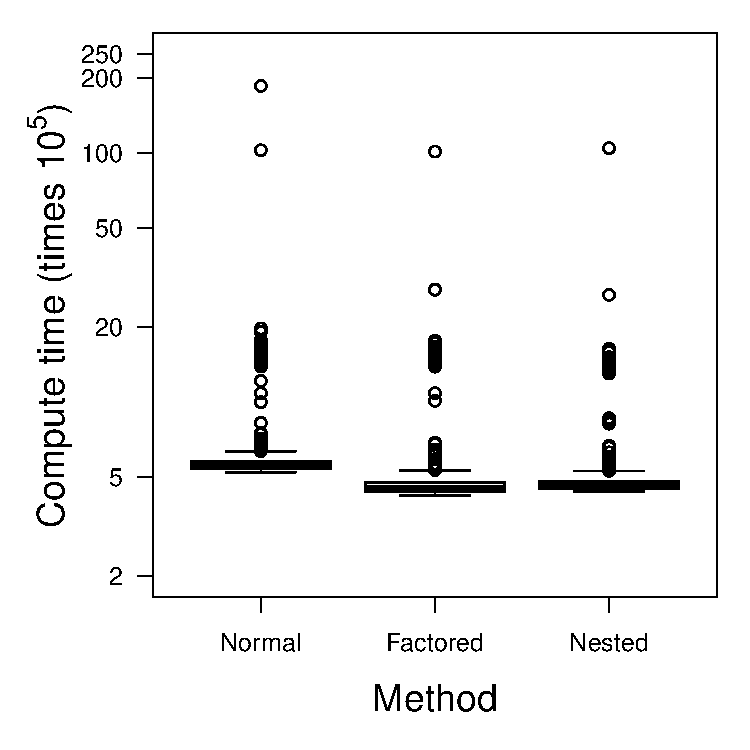
\includegraphics[width=0.5\textwidth]{1_basics/polynomial_evaluation_plot.pdf}
\caption{Median computing times (measured execution time in microseconds) are 607.1064 for~\(f_1\), 511.8887 for~\(f_2\), and 516.9337 for~\(f_3\).}\label{fig::polys}
\end{figure}


\noindent With respect to class, you might ask yourself why we have emphasized nesting, but not factoring, when it comes to working with polynomials.

%%%%%%%%%%%%%%%%%%%%%%%%%%%%%%%%%%%%%%
%%%%%%%%%%%%%%%%%%%%%%%%%%%%%%%%%%%%%%
\clearpage
\section{Root-finding and fixed-point problems}
\subsection{Fixed-point iteration}

Consider the function \[g(x) = 2^{-x} = e^{-\ln(2)x}\] and the associated fixed-point problem \(g(x) = x\). The result obtained by cobwebbing (graphically) is shown in the figure below, with the iterates marked in ticks on the bottom axis. Beyond \(n=4\) things get pretty crowded near the fixed point.
%
\begin{figure}[ht!]\centering
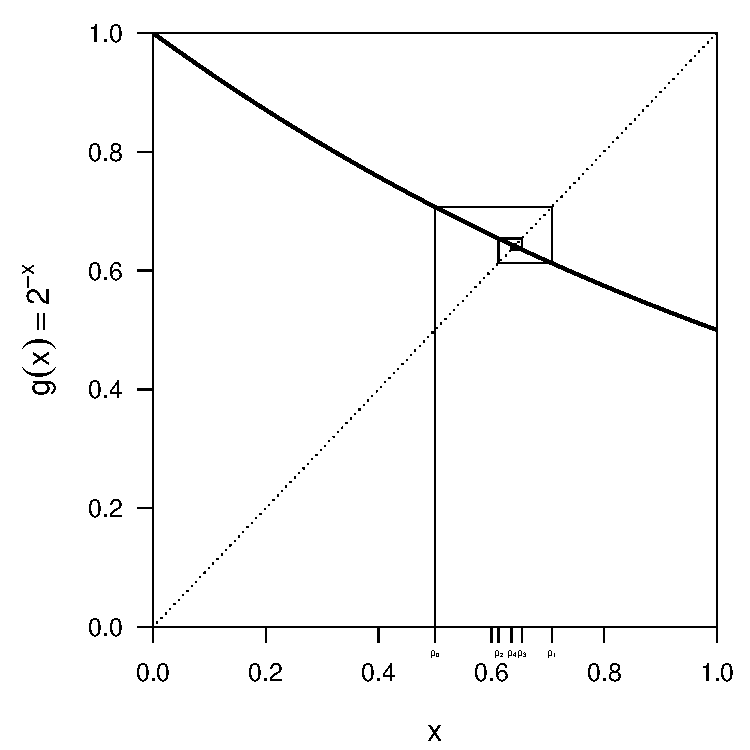
\includegraphics[width=0.5\textwidth]{1_basics/fixedpoint.pdf}
\caption{A fixed-point problem.}\label{fig::fpp}
\end{figure}
%
As tabular output we have the first few steps as well. Note that \(p_n\) are approximates to the root \(p\).
\begin{center}
\begin{tabular}{cc}
\(n\) & \(p_n\)\\
\hline\hline
0 & 0.5000000\\
1 & 0.7071068\\
2 & 0.6125473\\
3 & 0.6540409\\
4 & 0.6354978
\end{tabular}
\end{center}

Now, for a given degree of accuracy, how many iterations do we actually need? Consider \[2^{-x}=x\text{ on }\left[\frac{1}{3}, 1\right]\] The bounds are given by \[|p_n-p|\leq k^n \max(p_0-a, b - p_0)\]
using the initial guess, and by \[|p_n-p|\leq\frac{k^n}{1-k}|p_1-p_0|\] using the initial guess and first iteration. We will look at a few applications of the bounds to the problem above. First notice that \(g'(x) = -\ln(2)2^{-x}\) and \(|g'(x)| \leq \ln(2)2^{-{1}/{3}} < k = 0.551\), where \(k = 0.551\) is a bound on the magnitude of \(g'(x)\).

The worst possible initial guess would be at one of the endpoints, so we will start there (this maximizes the term \( \max(p_0-a, b - p_0)\), which in this case we actually want to do in order to generate a conservative bound). Taking \(D\) as the desired accuracy (i.e., an accuracy within \(10^{-D}\)), this gives, 
\begin{align*}
k^n \max(p_0-a, b - p_0) & < 10^{-D}\\
(0.551)^n \left(\frac{2}{3}\right) & < 10^{-D}\\
(0.551)^n & < \left(\frac{3}{2}\right)10^{-D}\\
n \log(0.551) & < \log\left(\frac{3}{2}\right) - D\\
n & > \frac{\log\left(\frac{3}{2}\right) - D}{\log(0.551)}
\end{align*}
In the last line, the inequality has been reversed since we are dividing by a negative. With \(D=4\) this gives \(n > 14.77277\) which requires \(N=15\) steps.

For the second bound, we actually need \(p_1\) in addition to \(p_0\). From \(p_0 = \frac{2}{3}\), we have \(p_1 = 2^{-1/3}\) (so \(|p_1-p_0| = |2^{-1/3} - \frac{1}{3}| ~\approx~ 0.4604\)). Similarly, from \(p_0=1\), we have \(p_1 = \frac{1}{2}\) (so \(|p_1-p_0| = |\frac{1}{2} - 1| = 0.5\)). We will use the second of these which is larger in value.
\begin{align*}
\frac{k^n}{1-k}|p_1-p_0| & < 10^{-D}\\
\frac{(0.551)^n}{1-0.551}(0.5) & < 10^{-D}\\
(0.551)^n & < \left(\frac{1-0.551}{0.5}\right) 10^{-D}\\
n\log(0.551) & < \log\left(\frac{1-0.551}{0.5}\right) -D\\
n & > \frac{\log\left(\frac{1-0.551}{0.5}\right) -D}{\log(0.551)}\\
\end{align*}
For consistency, with \(D=4\) this gives \(n > 15.63357\) which requires \(N=16\) steps. We have to do at least \(16\) steps to ensure we are within the bound, though we may satisfy this much more quickly. Notice that this is quite a bit more work than our bound for the Bisection method required.

%%%%%%%%%%%%%%%%%%%%%%%%%%%%%%%%%%%%%%

Consider the root-finding problem \(f(x) = x^4-3x^2-3\). It has many different, but equivalent, fixed-point problems.
\begin{align*}
g_1(x) & = x- f(x) = x\\
g_2(x) & = x+f(x) = x\\
g_3(x) & = \sqrt{\frac{3}{x^2-3}} = x\\
g_4(x) & = x - \frac{x^4-3x^2-3}{4x^3-6x}
\end{align*}

\begin{center}
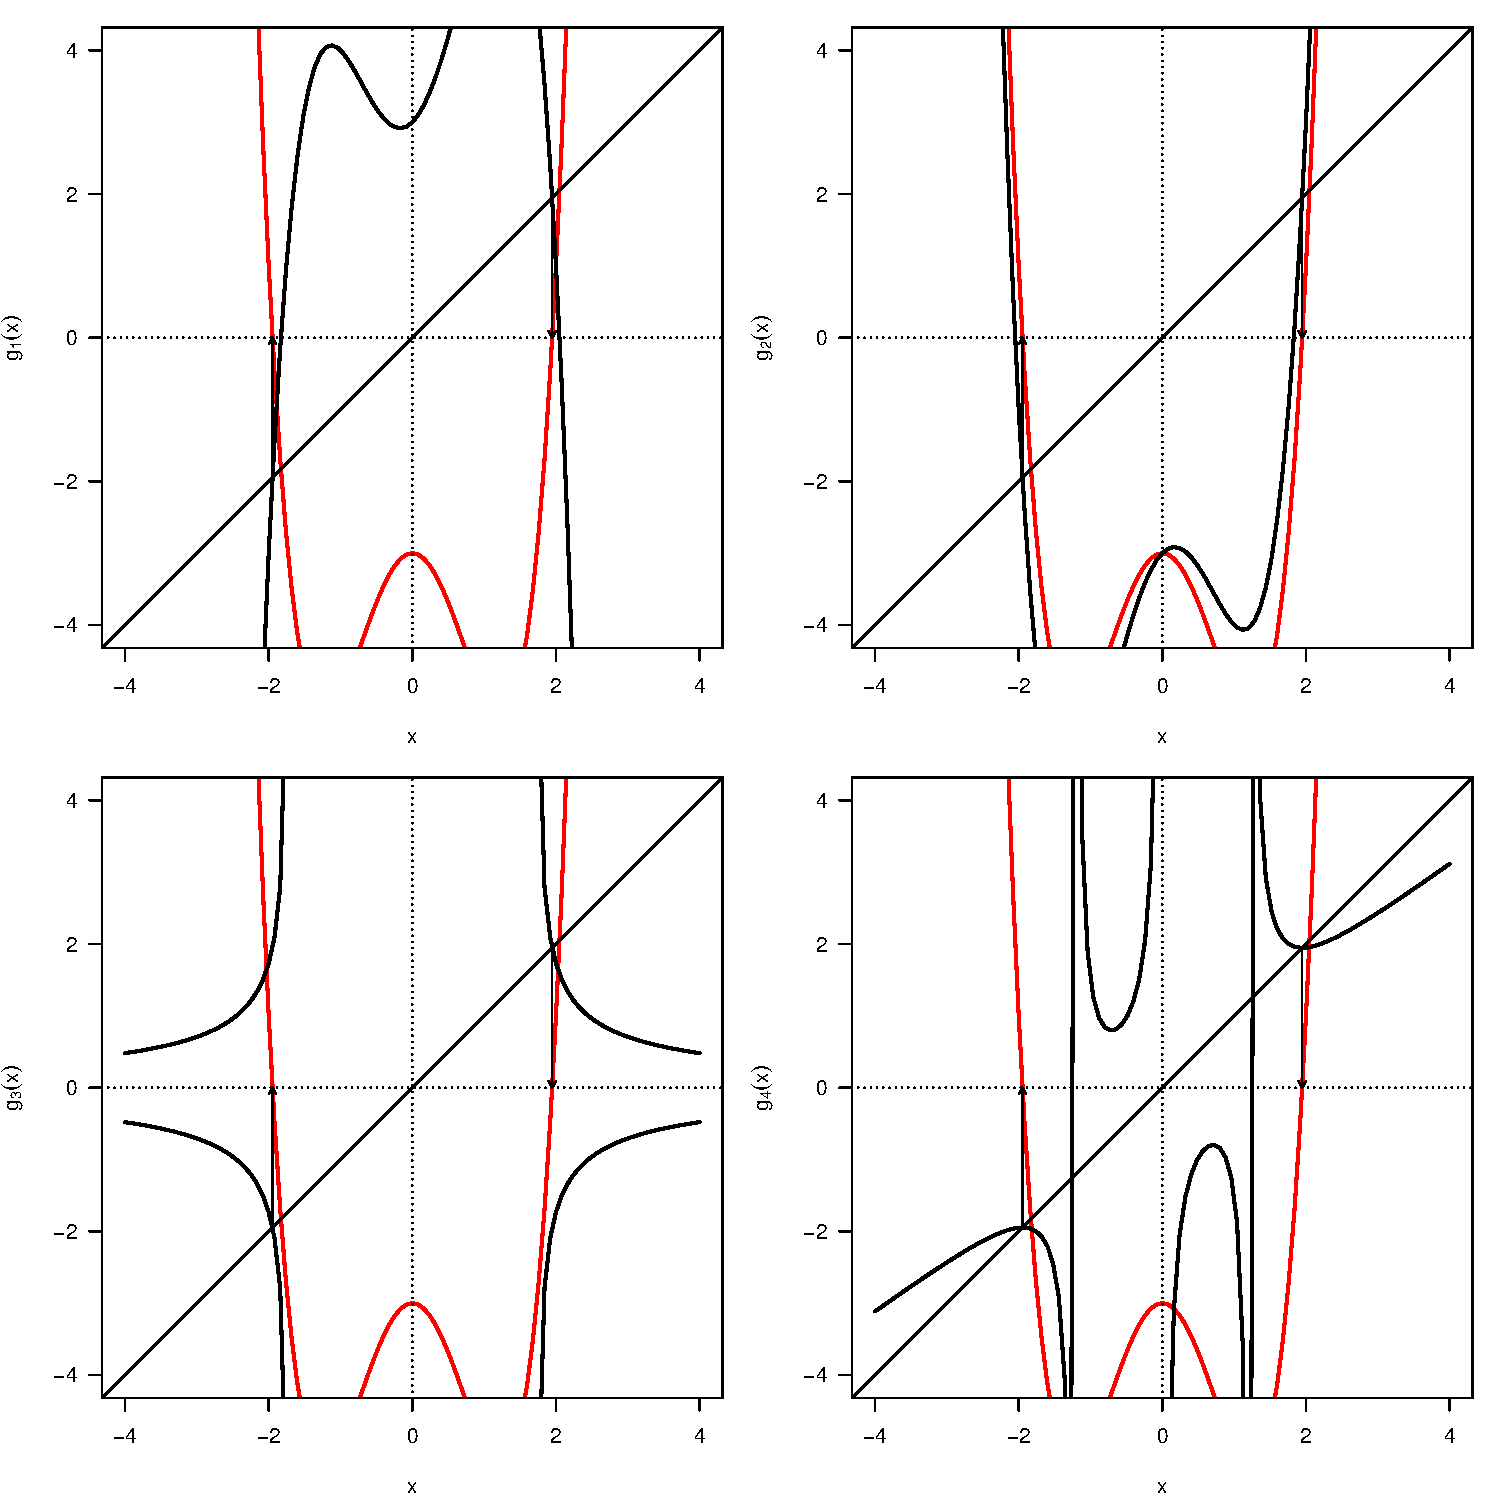
\includegraphics[width=\textwidth]{1_basics/bad.pdf}
\end{center}

\newpage
A better formulation is given by \[g_5(x) = \sqrt[4]{3x^2+3}\]

\begin{center}
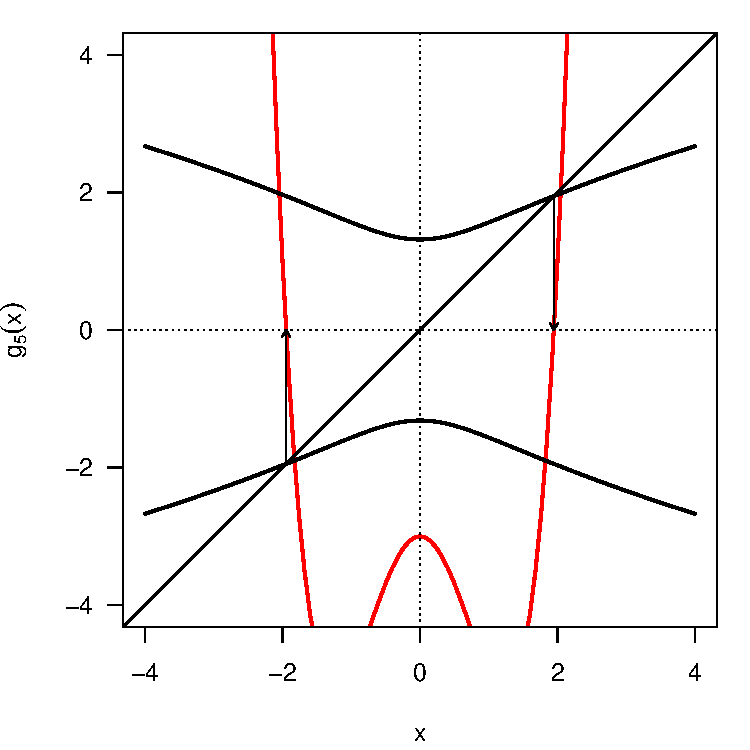
\includegraphics[width=0.5\textwidth]{1_basics/good.pdf}
\end{center}

%%%%%%%%%%%%%%%%%%%%%%%%%%%%%%%%%%%%%%
%%%%%%%%%%%%%%%%%%%%%%%%%%%%%%%%%%%%%%
Consider the root-finding problem \(3x^2-e^x = 0\). It has a few different, but equivalent, fixed-point problems.
\begin{align}
g_1(x) & = \pm\sqrt{\dfrac{e^x}{3}} = x\\
g_2(x) & = \ln(3x^2) = x\\
g_3(x) & = 3x^2 - e^x + x = x
\end{align}
Unfortunately these differ with regard to theory of fixed-point iterations. In particular, keep in mind
\begin{description}
\item[for existence:] the trapping region \(g\in[a,b]\) for \(x\in[a,b]\)
\item[for uniqueness:] the slope criterion \(0<|g'(x)|<1\)
\end{description}

The first function, \(g_1(x)\) is able to capture two of the three points of interest, with nicely trapped solutions and small derivatives on those intervals. It does fail to capture the third (rightmost) root, where the slope exceeds one (see Fig.~\ref{fig::g1}). Though our intervals cannot include \(x=0\), \(g_2(x)\) works well for the largest root, where the derivative is small and the appropriate trapping region can be constructed (see Fig.~\ref{fig::g2}). The simplest formulation algebraically is \(g_3(x)\), yet this has by far the worst characteristics with respect to the fixed-point theory for existence and uniqueness (see Fig.~\ref{fig::g3}). It is difficult to constrict suitable trapping regions and there are only narrow ranges for which the derivative is appropriately bounded in magnitude. 

\begin{figure}[ht!]
\begin{minipage}{0.48\textwidth}
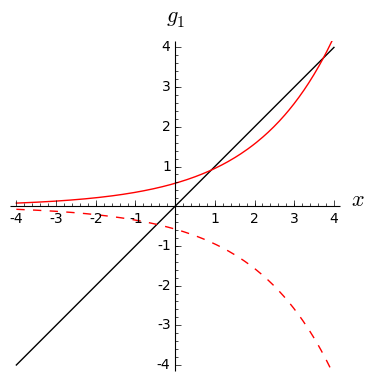
\includegraphics[width=\textwidth]{1_basics/g1.png}
\end{minipage}
\begin{minipage}{0.48\textwidth}
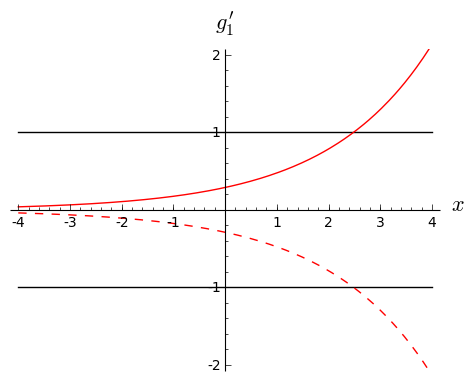
\includegraphics[width=\textwidth]{1_basics/g1p.png}
\end{minipage}
\caption{Two functions that give rise to fixed-point problems. Dotted corresponds to the negative value of the square root and the solid line corresponds to the positive value. Left: intersections of each with the black \(1:1\) line indicate fixed points. Right: values between \(-1\) and \(1\) indicate that a fixed point, if it exists, is unique.}\label{fig::g1}
\end{figure}

\begin{figure}[ht!]
\begin{minipage}{0.48\textwidth}
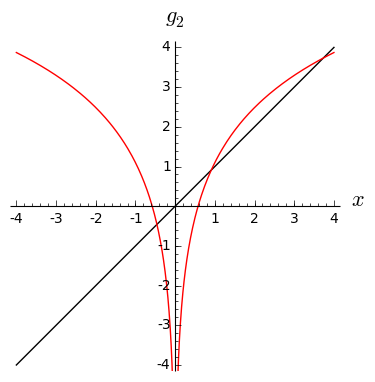
\includegraphics[width=\textwidth]{1_basics/g2.png}
\end{minipage}
\begin{minipage}{0.48\textwidth}
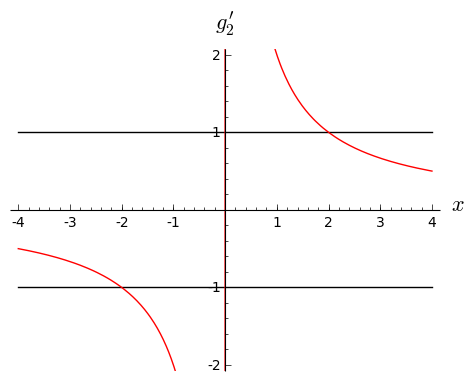
\includegraphics[width=\textwidth]{1_basics/g2p.png}
\end{minipage}
\caption{Left: intersections with the black \(1:1\) line indicate fixed points. Right: values between \(-1\) and \(1\) indicate that a fixed point, if it exists, is unique. Notice that the smaller the value of the fixed point, the steeper the function \(g_2(x)\).}\label{fig::g2}
\end{figure}

\begin{figure}[hb!]
\begin{minipage}{0.48\textwidth}
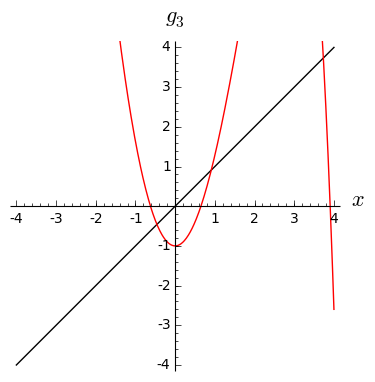
\includegraphics[width=\textwidth]{1_basics/g3.png}
\end{minipage}
\begin{minipage}{0.48\textwidth}
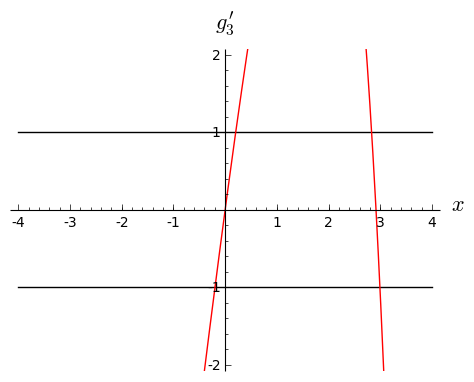
\includegraphics[width=\textwidth]{1_basics/g3p.png}
\end{minipage}
\caption{Left: intersections with the black \(1:1\) line indicate fixed points. Right: values between \(-1\) and \(1\) indicate that a fixed point, if it exists, is unique.}\label{fig::g3}
\end{figure}

%%%%%%%%%%%%%%%%%%%%%%%%%%%%%%%%%%%%%%
%%%%%%%%%%%%%%%%%%%%%%%%%%%%%%%%%%%%%%

Consider the fixed-point problems \(\sin(x) = x\) (below, left) and \(\cos(x) = x\) (below, right).
%
\begin{figure}[hb!]\centering
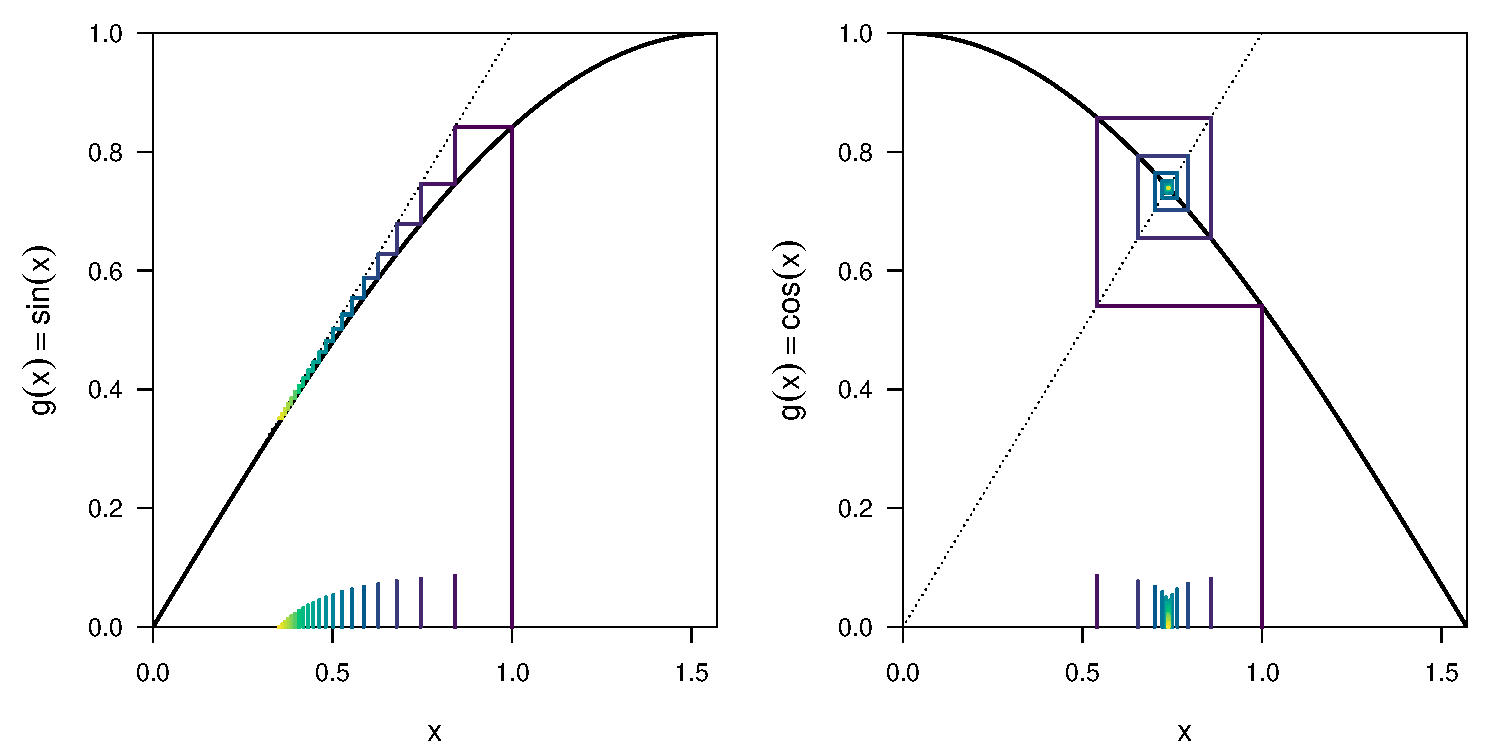
\includegraphics[width=0.95\textwidth]{1_basics/fixpt_trig.pdf}
\caption{A trigonometric fixed-point problem.}\label{fig::trigfpp}
\end{figure}

A total of \(20\) iterations of each problem are shown in the color figure above. Time is indicated in two ways: on the graph early steps are in dark blue and fade to yellow. Along the axis earlier approximations are marked by tall (also dark blue) tick marks and later iterations are marked by shorter (also yellow) tick marks. The scaling of the above-axis tick marks is nothing quantitative or necessarily related to the values of the approximation itself, it is just meant to show the progression of the iterations.

For two problems starting from \(p_0=1\), we see the iterations approaching the fixed point visible on each panel of the graph. Solutions to the first fixed-point problem (left) converge very slowly, while those to the second (right) converge very quickly. Details of the approaches to the fixed points are interesting as well. Approximations converging to the true solution of \(p=0\) for the first problem decrease monotonically, while those converging to the true solution of the second problem oscillate.

\paragraph{Challenge} For each of the above, state an associated rootfinding problem, an interval on which you could apply the bisection method, and the number of iterations it would take to approximate the root to an accuracy of \(10^{-6}\) with bisection.

%%%%%%%%%%%%%%%%%%%%%%%%%%%%%%%%%%%%%%
\clearpage
\section{Interpolation and approximation}
\subsection{Polynomial interpolation}
\subsubsection{Lagrange interpolation}
Below are \(L_k(x) = L_{7, k}(x)\) for \(8\) equally spaced points \(x_0 = -1, \dots, x_7 = 1\) on \([-1, 1]\). 

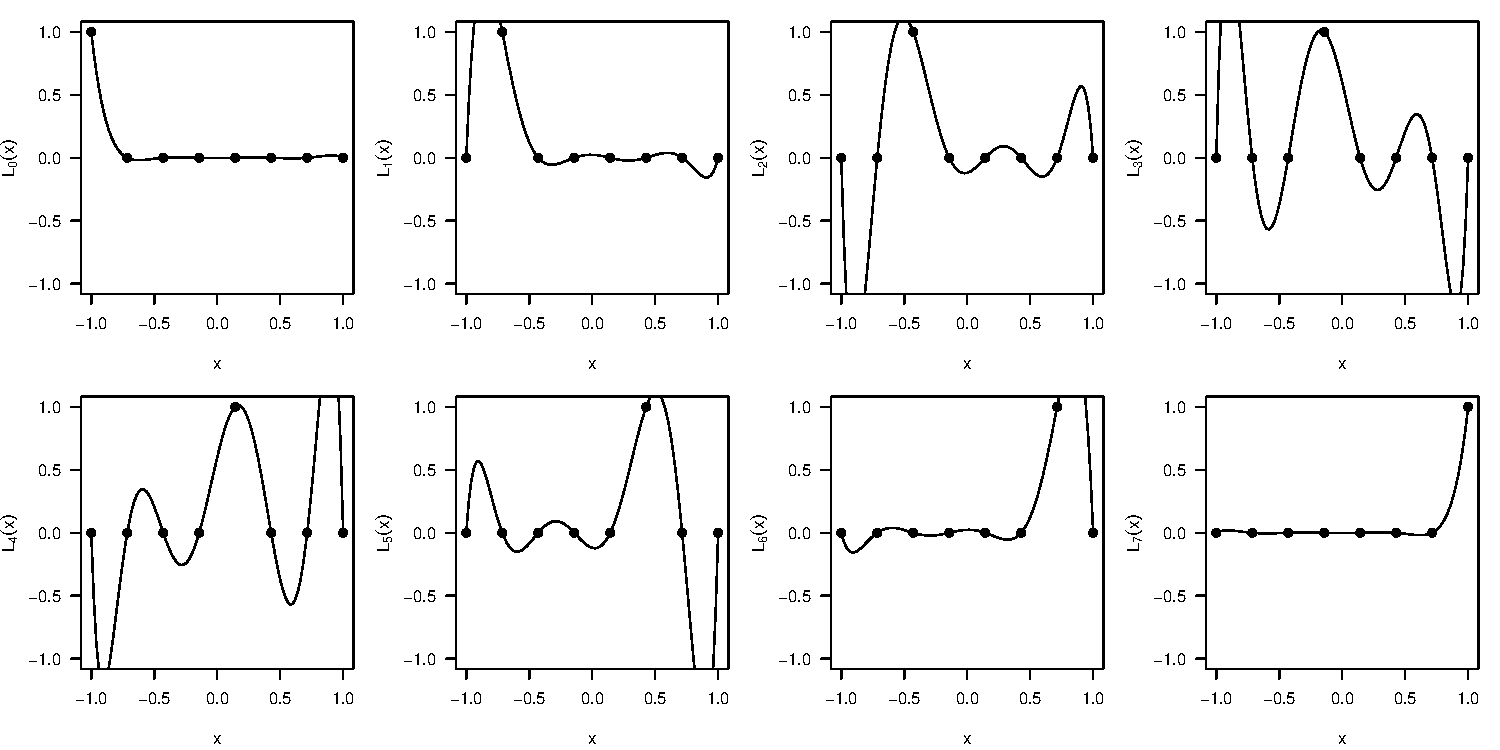
\includegraphics[width=\textwidth]{2_interpolation/Li.pdf}

Considering the function \[f(x) = x^3e^{-1.1x}\sin(x)\] we show the approximation \[P(x) = P_7(x) = \sum_{k=0}^7 f(x_k)L_k(x)\] (along with the function) on the left and the error on the right.

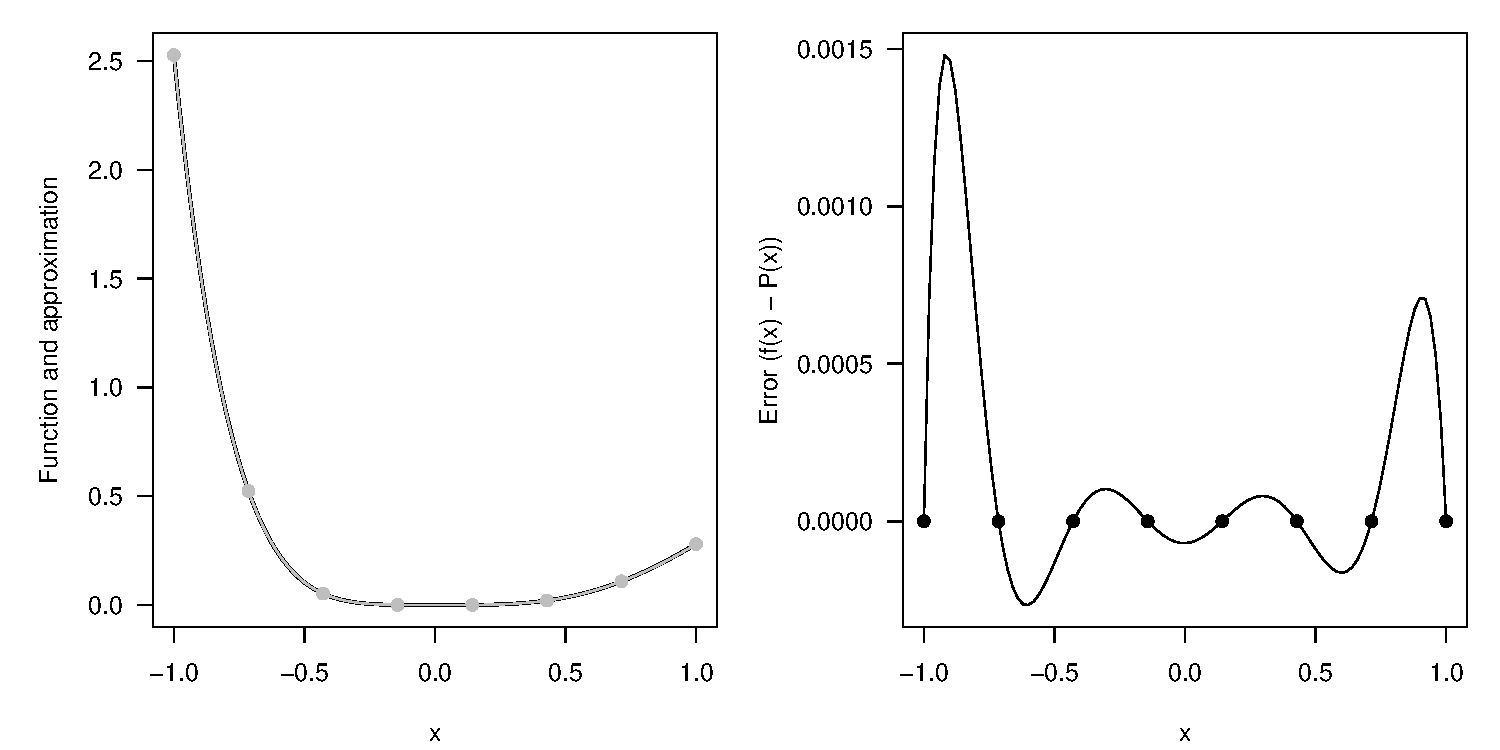
\includegraphics[width=\textwidth]{2_interpolation/fP.pdf}

%%%%%%%%%%%%%%%%%%%%%%%%%%%%%%%%%%%%%%
%%%%%%%%%%%%%%%%%%%%%%%%%%%%%%%%%%%%%%
\subsubsection{Cubic spline interpolation}
\begin{description}
\item[Note:] Before you begin, please note that there is a typo in the clamped spline example in the book (Example 2, page 148, eighth edition), the correct solution will be given below.

\item[Intro:] When computing a cubic spline with \(n+1\) grid points, keep in mind that we have \(n\) intervals, \(n\) spline segments, and an \((n+1)\times (n+1)\) matrix. For example, if the data is known at the grid points \(x_0, x_1, x_2, x_3, x_4\) we have \(5\) points, \(4\) intervals, \(4\) spline segments, and a \(5\times5\) matrix. The spacings between grid points, defined \(h_j = x_{j+1} - x_j\), are used below.

\item[General approach:] We can verify the conditions of the spline by definition, but ultimately the way to implement this, even for small datasets, is to use matrix algebra. Let's use the vector \(\mathbf{r}\) (as in \(\textbf{A}\textbf{x} = \textbf{r}\), rather than \(\textbf{A}\textbf{x} = \textbf{b}\)) for the right-hand side to avoid likely confusion between entries of the right-hand side vector and the coefficients \(b_j\) of the splines. The first and last rows of \(\mathbf{A}\) and \(\mathbf{r}\) depend on the choice of boundary conditions, but the interior rows are illustrated below. On the interior rows of the main diagonal, \(\mathbf{A}\) has entries \[2(h_0+h_1), 2(h_1 + h_2), \cdots, 2(h_{n-3} + h_{n-2}), 2(h_{n-2} + h_{n-1})\] On the interior rows of the sub-diagonal (below main), \(\mathbf{A}\) has entries \[h_0, h_1, \cdots, h_{n-3}, h_{n-2}\] On the interior rows of the super-diagonal (above main), \(\mathbf{A}\) has entries \[h_1, h_2, \cdots, h_{n-2}, h_{n-1}\] 

\begin{align*}
\mathbf{A} & = \setcounter{MaxMatrixCols}{20}
\begin{bmatrix}
\cdot & \cdot & \cdot & \cdot & \cdot & \cdot & \cdot & \cdot & \cdot &\cdot & \cdot \\
h_0 & 2(h_0+h_1) & h_1 & 0 & \cdot & \cdot & \cdot& \cdot & \cdot &\cdot & 0\\
\cdot & \ddots & \ddots & \ddots & \cdot & \cdot & \cdot & \cdot & \cdot &\cdot & \cdot \\
0 & \cdot & \cdot & 0 & h_{j-1} & 2(h_{j-1}+h_{j}) & h_{j} & 0 & \cdot & \cdot & 0\\
\cdot & \cdot & \cdot & \cdot & \cdot & \cdot & \cdot & \cdot & \cdot &\cdot & \cdot \\
0 & \cdot & \cdot & \cdot& \cdot & \cdot &\cdot & 0 & h_{n-2} & 2(h_{n-2}+h_{n-1}) & h_{n-1}\\
\cdot & \cdot & \cdot & \cdot & \cdot & \cdot & \cdot & \cdot & \cdot &\cdot & \cdot \\
\end{bmatrix}\\
\mathbf{x} & = 
\left[\begin{array}{c}
c_0 \\
c_1 \\
\vdots \\
c_{n-1} \\
c_n \\
\end{array}\right]\\
\mathbf{r} & = 
\left[\begin{array}{c}
\cdots \\
3\left(\dfrac{a_2-a_1}{h_1} - \dfrac{a_1-a_0}{h_0}\right) \\
\vdots \\
3\left(\dfrac{a_n-a_{n-1}}{h_{n-1}} - \dfrac{a_{n-1}-a_{n-2}}{h_{n-2}}\right) \\
\cdots \\
\end{array}\right]
\end{align*}
\item[Natural BCs:] The interior rows of \(\mathbf{A}\) are as described above, but the first row begins with \(1, 0, \dots\) and the last row ends with \(\dots, 0, 1\). To satisfy the boundary condition, the first and last rows of of \(\mathbf{r}\) are exactly \(0\).
\begin{align*}
\mathbf{A} & = \setcounter{MaxMatrixCols}{20}
\begin{bmatrix}
1 & 0 & \cdot & \cdot & \cdot & \cdot & \cdot & \cdot & \cdot &\cdot & \cdot \\
\cdot & \cdot & \cdot & \cdot & \cdot & \cdot & \cdot & \cdot & \cdot &\cdot & \cdot \\
\vdots & \vdots & \vdots & \vdots & \vdots & \vdots & \vdots & \vdots & \vdots &\vdots & \vdots \\
\cdot & \cdot & \cdot & \cdot & \cdot & \cdot & \cdot & \cdot & \cdot &\cdot & \cdot \\
\cdot & \cdot & \cdot & \cdot & \cdot & \cdot & \cdot & \cdot & \cdot &0 & 1 \\
\end{bmatrix}\\
\mathbf{r} & = 
\left[\begin{array}{c}
0 \\
\vdots \\
\vdots \\
\vdots\\
0 \\
\end{array}\right]
\end{align*}
\item[Clamped BCs:] The interior rows of \(\mathbf{A}\) are as described above, but the first row begins with \(2h_0, h_0, 0, \dots\) and the last row ends with \(\dots, 0, h_{n-1}, 2h_{n-1}\). To satisfy the boundary condition, the first and last rows of of \(\mathbf{r}\) are exactly \(3\left(\dfrac{a_1-a_0}{h_0} -f'(a)\right)\) and \(3\left(f'(b) - \dfrac{a_n-a_{n-1}}{h_{n-1}}\right)\), respectively.

\begin{align*}
\mathbf{A} & = %\setcounter{MaxMatrixCols}{20}
\begin{bmatrix}
2h_0 & h_0 & 0 &\cdot & \cdot & \cdot &\cdot & 0 \\
\cdot & \ddots & \ddots & \ddots & \cdots & \cdots &\cdots & \vdots \\
%\vdots & \ddots & \vdots & \vdots & \vdots & \vdots &\vdots & \vdots \\
\vdots & \cdots & \cdots & \cdots & \ddots & \ddots &\ddots & \cdot \\
\cdot & \cdots & \cdot & \cdot & \cdot & 0 &h_{n-1} & 2h_{n-1} \\
\end{bmatrix}\\
\mathbf{r} & = 
\left[\begin{array}{c}
3\left(\dfrac{a_1-a_0}{h_0} -f'(a)\right) \\
\vdots \\
\vdots \\
\vdots\\
3\left(f'(b) - \dfrac{a_n-a_{n-1}}{h_{n-1}}\right) \\
\end{array}\right]
\end{align*}

\item[Parameterizing the spline:] Once the \(c_j\)'s have been solved, the \(b_j\)'s and \(d_j\)'s can be specified \textit{in reverse order} from \(j=n-1,n-2,\dots,0\) (see Alg.~3.4 (Step 6) or Alg.~3.5 (Step 7)).
\begin{align*}
b_j & = \dfrac{a_{j+1} - a_j}{h_j} - \dfrac{h_j(c_{j+1} + 2c_j)}{3}\\
d_j & = \dfrac{c_{j+1} - c_j}{3h_j}
\end{align*}
Notice that \(c_n\) (from \(\mathbf{x}\)) is used in the calculation of \(d_{n-1}\), but is never actually used in a spline. Regardless of the boundary condition, the calculated coefficients will appear in the spline of the form
%
\begin{equation*}
S(t) = \left\{\begin{alignedat}{2}
&\phantom{a_j + b_j(x-x_j) + } \cdots \phantom{(x-x_j)^2 + d_j(x-x_j)^3}, &&\cdots\\
S_j(t) &= a_j + b_j(x-x_j) + c_j(x-x_j)^2 + d_j(x-x_j)^3, \quad &&x_j\leq x < x_{j+1}\\
&\phantom{a_j + b_j(x-x_j) + } \cdots \phantom{(x-x_j)^2 + d_j(x-x_j)^3}, &&\cdots\\
\end{alignedat}\right.
\end{equation*}
%
Note that \(x_0=a\) and \(x_n=b\).
\item[Keep reading:] (next page, please)
\newpage

\item[Example] Consider the data \(x_0 = 0, x_1=1, x_2, =2, x_3=3\) and \(f(x) = e^x\). 

\begin{description}
\item[A natural spline:] See Example 1 on page 143.
\begin{center}
\begin{tabular}{c|cccc}
\(j\) & \(a_j\) & \(b_j\) & \(c_j\) & \(d_j\)\\
\hline
\hline
0 & 1.000000 & 1.465998 & 0.0000000 & 0.2522842\\
1 & 2.718282 & 2.222850 & 0.7568526 & 1.6910714\\
2 & 7.389056 & 8.809770 & 5.8300668 & -1.9433556
\end{tabular}

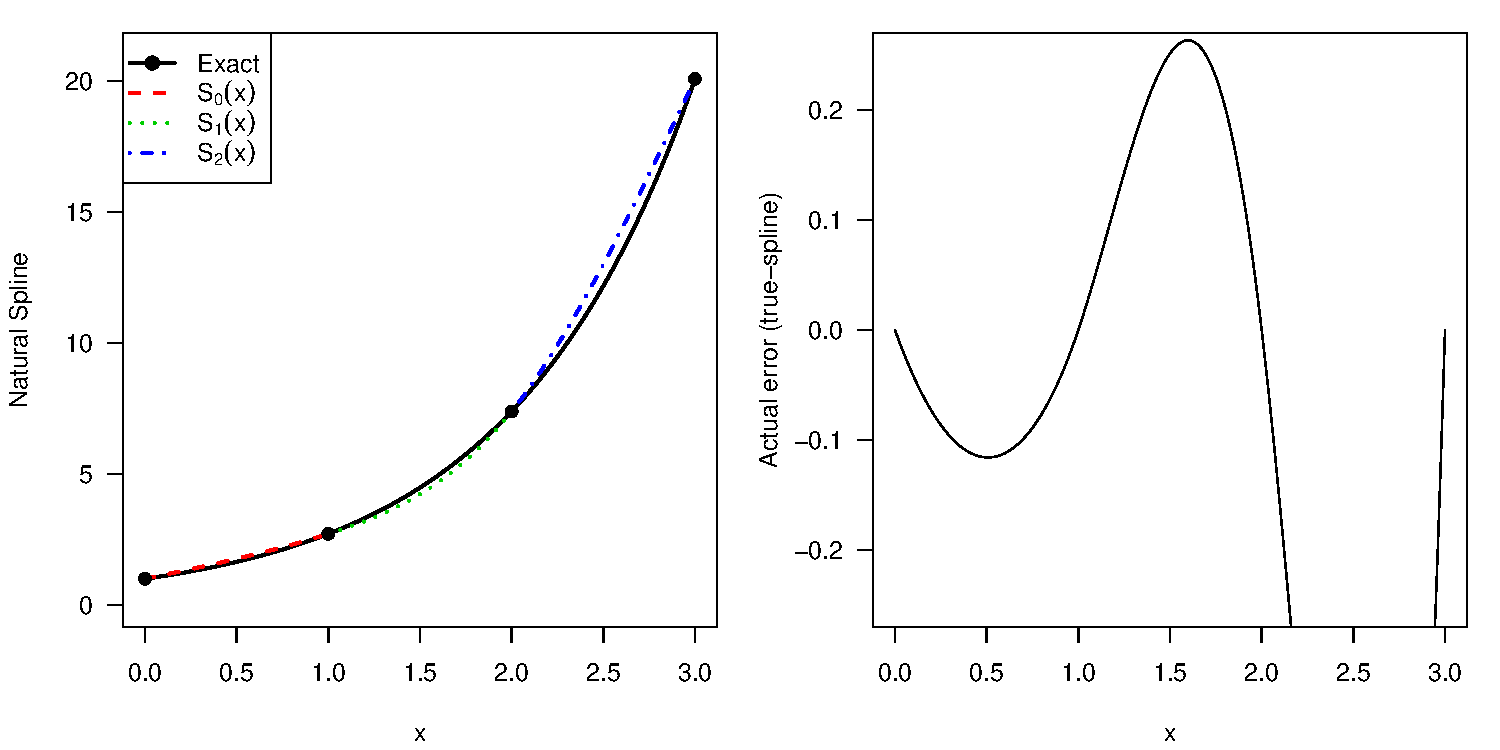
\includegraphics[width=0.9\textwidth]{2_interpolation/natural.pdf}
\end{center}

\vfill

\item[A clamped spline:] See Example 2 on page 148.
\begin{center}
\begin{tabular}{c|cccc}
\(j\) & \(a_j\) & \(b_j\) & \(c_j\) & \(d_j\)\\
\hline
\hline
0 & 1.000000 & 1.000000 & 0.4446825 & 0.2735993\\
1 & 2.718282 & 2.710163 & 1.2654805 & 0.6951308\\
2 & 7.389056 & 7.326516 & 3.3508729 & 2.0190916
\end{tabular}

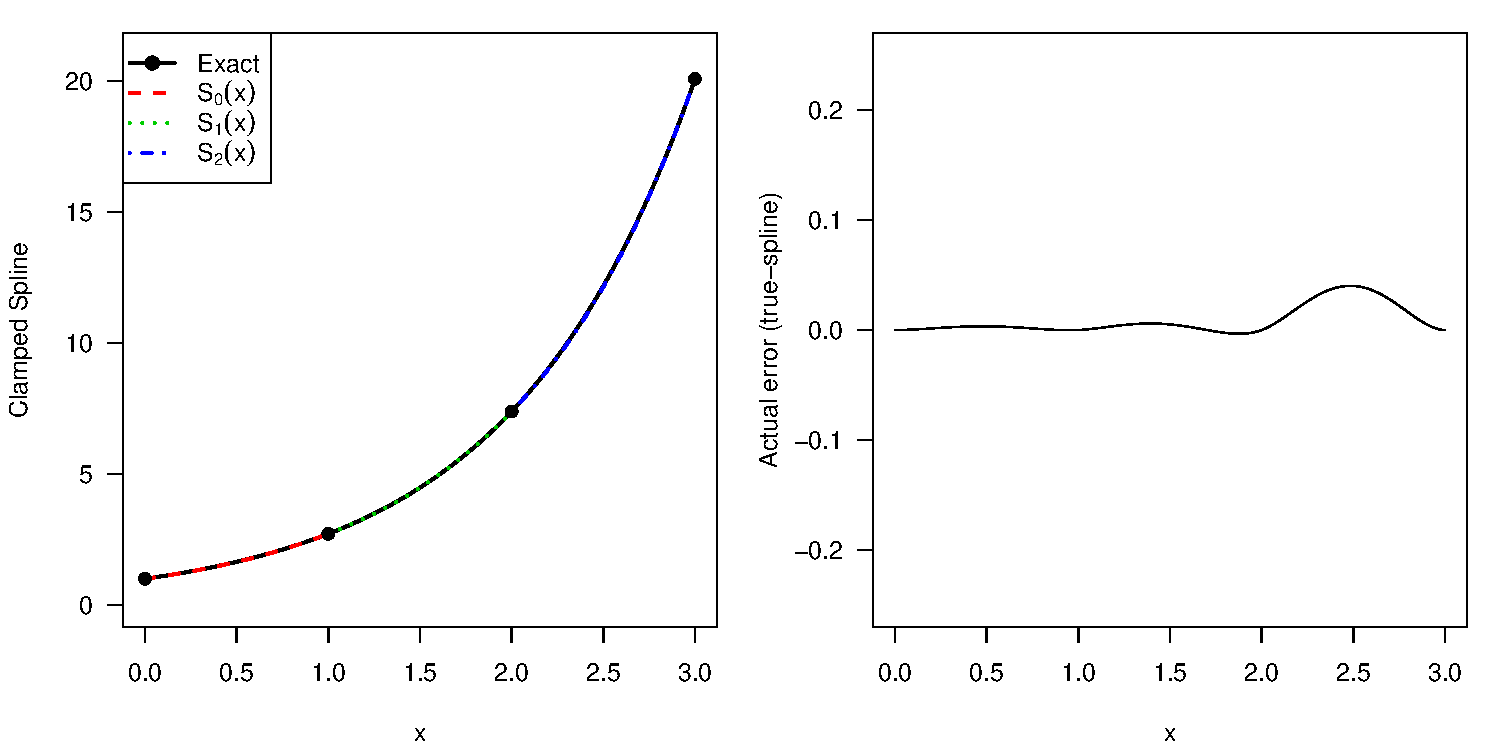
\includegraphics[width=0.9\textwidth]{2_interpolation/clamped.pdf}

\end{center}
\end{description}
\end{description}

%%%%%%%%%%%%%%%%%%%%%%%%%%%%%%%%%%%%%%
%%%%%%%%%%%%%%%%%%%%%%%%%%%%%%%%%%%%%%
\subsection{Discrete least squares approximation}

Given the data in the vehicle speed problems (see sections 3.3, 3.4 homework), we can plot a few functions representing the position data (see Figure~\ref{fig::speed_plots}). The Hermite (black) and spline (red) interpolations exactly pass through the position data points. On the other hand, the linear approximation (blue) does not exactly pass through a single of these points.
%
\begin{figure}[ht!]\centering
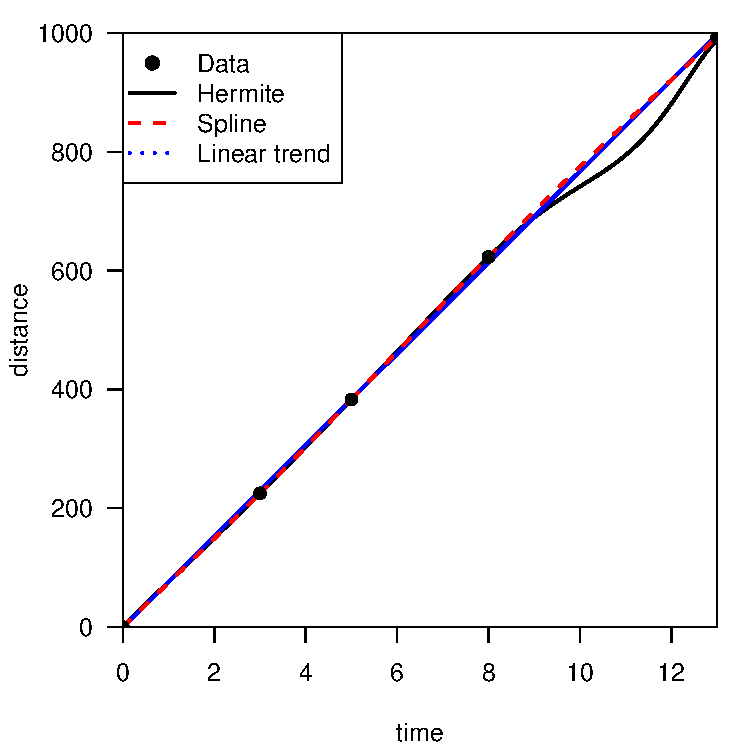
\includegraphics[width=0.5\textwidth]{3_approximation/speed1.pdf}
\caption{Data and interpolating and approximating polynomials.}\label{fig::speed_plots}
\end{figure}

\begin{figure}[ht!]\centering
\begin{minipage}{0.48\textwidth}
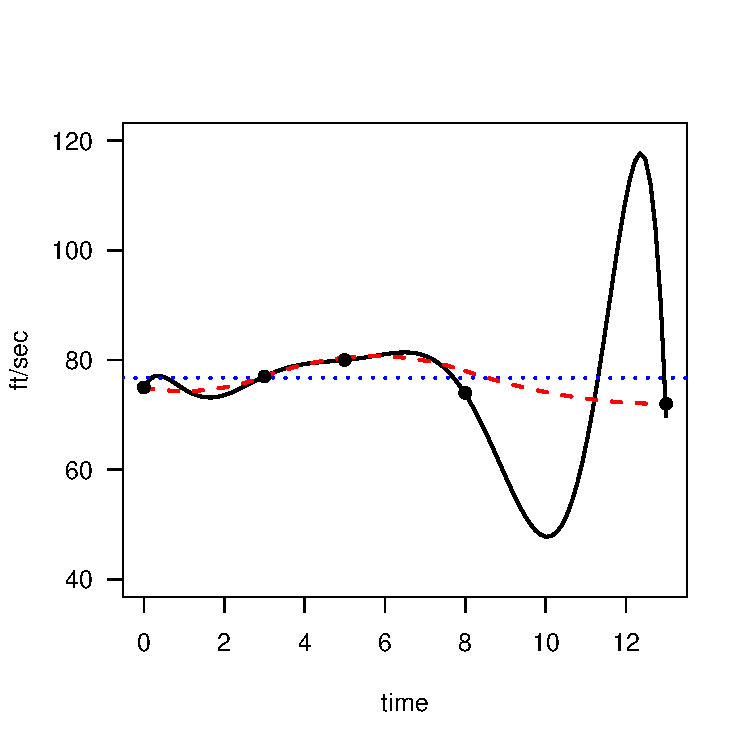
\includegraphics[width=\textwidth]{3_approximation/speed2.pdf}

\end{minipage}
\begin{minipage}{0.48\textwidth}

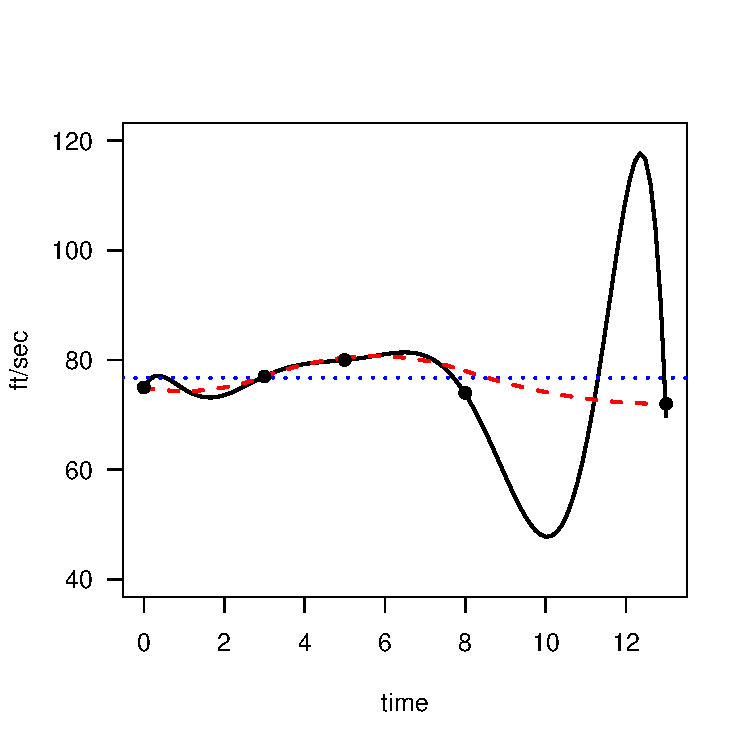
\includegraphics[width=\textwidth]{3_approximation/speed2.pdf}
\end{minipage}

\caption{Speed data and predicted speed by interpolating and approximating polynomials (\textbf{left:} feet per second and~\textbf{right:} miles per hour).}\label{fig::speed_plots2}
\end{figure}

\noindent There are a variety of factors to weigh when choosing a method for representing data by a function.

%%%%%%%%%%%%%%%%%%%%%%%%%%%%%%%%%%%%%%
%%%%%%%%%%%%%%%%%%%%%%%%%%%%%%%%%%%%%%

\subsection*{Discrete case (i.e., 8.1, pg. 486)}
Consider the last term \[\sum_{i=1}^m\Big(P_n(x_i)\Big)^2 = \sum_{i=1}^m \left(\sum_{j=0}^n a_j x_i^j\right)^2\] in the definition of the error \(E = E_2(a_0, a_1, \dots, a_n)\) for discrete least squares approximation. We have the following (though I do not find this particularly illuminating and instead prefer to differentiate before addressing the sums), where it might initially be helpful to remember that \(x_i^0 = 1\) and \(x_i^1 = x_i\) (e.g., \(a_0 x_i^0 = a_0\cdot1 =a_0\) and \(a_1 x_i^1 = a_1x_i\)), 
\begin{align*}
 \sum_{i=1}^m \left(\sum_{j=0}^n a_j x_i^j\right)^2 & = \sum_{i=1}^m (a_0 + a_1x_i+ \dots + a_n x_i^n)(a_0 + a_1x_i + \dots + a_n x_i^n)\\
 & = \sum_{i=1}^m \Big[a_0 (a_0 + \dots + a_n x_i^n) + \dots + a_jx_i^j(a_0 + \dots + a_n x_i^n) + \dots + a_n x_i^n(a_0 + \dots + a_n x_i^n)\Big]\\
 & = \sum_{i=1}^m \sum_{j=0}^n a_jx_i^j(a_0 + a_1x_i + \dots + a_n x_i^n)\\
 & = \sum_{j=0}^n a_j \sum_{i=1}^m x_i^j(a_0 + a_1x_i + \dots + a_n x_i^n)\\
 & = \sum_{j=0}^n a_j \sum_{i=1}^m x_i^j \sum_{k=0}^n a_k x_i^k\\
 & = \sum_{j=0}^n a_j \sum_{i=1}^m \sum_{k=0}^n a_k x_i^{j+k}\\
% & = \sum_{j=0}^n a_j \sum_{k=0}^n a_k \sum_{i=1}^m x_i^{j+k}\\
% & = \sum_{i=1}^m \sum_{j=0}^n a_jx_i^j \sum_{k=0}^n a_kx_i^k\\
 % & = \sum_{i=1}^m a_0 a_0 + (a_0a_1 + a_1a_0)x_i + (a_0a_2+a_1a_1+a_2a_0)x_i^2 + \dots\\
% & = \sum_{i=1}^m a_0 a_0 + (a_0a_1 + a_1a_0)x_i + (a_0a_2+a_1a_1+a_2a_0)x_i^2 + \dots\\
 & = \sum_{j=0}^n\sum_{k=0}^n a_ja_k\Big(\sum_{i=1}^m x_i^{j+k}\Big)
 \end{align*}
Our goal is the partial derivative of this term with respect to \(a_j\). Notice the following, where key steps are moving differentiation under the sum, applying the product rule, and rearranging the sum,
\begin{align*}
\dfrac{\partial}{\partial a_j} \left(\sum_{i=1}^m \left(\sum_{j=0}^n a_j x_i^j\right)^2 \right) & = \dfrac{\partial}{\partial a_j}\Big(\sum_{i=1}^m (a_0 + a_1x_i + \dots + a_n x_i^n)(a_0 + a_1x_i + \dots + a_n x_i^n)\Big)\\
& = \sum_{i=1}^m \dfrac{\partial}{\partial a_j}\Big((a_0 + a_1x_i + \dots + a_n x_i^n)(a_0 + a_1x_i + \dots + a_n x_i^n)\Big)\\
& = \sum_{i=1}^m \left(x_i^j(a_0 + a_1x_i + \dots + a_n x_i^n) + (a_0 + a_1x_i + \dots + a_n x_i^n) x_i^j\right)\\
& = \sum_{i=1}^m 2\left(x_i^j(a_0 + a_1x_i + \dots + a_n x_i^n)\right)\\
& = \sum_{i=1}^m 2\left(x_i^j\sum_{k=0}^n(a_kx_i^k)\right)\\
& = 2\sum_{k=0}^n a_k \sum_{i=1}^m x_i^{j+k}\\
%& = \int_a^b 2x_i^j(a_0 + a_1x_i + \dots + a_n x_i^n)\,dx_i\\
%& = 2\int_a^b x_i^j\sum_{k=0}^n a_k x_i^k\,dx_i\\
%& = 2\int_a^b \sum_{k=0}^n a_k x_i^{j+k}\,dx_i\\
%& = 2\sum_{k=0}^n a_k \int_a^b x_i^{j+k}\,dx_i
\end{align*}
Related to this, to find the least squares polynomial approximation to \(\{(x_i, y_i)\}_{i=1}^m\) by \(P_n(x)~=~\sum\limits_{k=0}^n a_k x^k\), we solve \[D^TD\vec{a} =D^T\vec{y}\] for the vector of unknown coefficients \(\vec{a}\) where \[D = \left[\begin{array}{cccc} (x_1)^0 & (x_1)^1 & \cdots & (x_1)^n\\
(x_2)^0 & (x_2)^1 & \cdots & (x_2)^n\\
\vdots & \vdots & \vdots & \vdots\\
(x_m)^0 & (x_m)^1 & \cdots & (x_m)^n
\end{array}\right]\]

\newpage

\subsection*{Continuous case (i.e., 8.2, pg. 495)}
Consider the last term \[\int_a^b \left(\sum_{k=0}^n a_k x^k\right)^2\] in the definition of the error \(E = E_2(a_0, a_1, \dots, a_n)\) for least squares polynomial approximation. We have,
\begin{align*}
\int_a^b \left(\sum_{k=0}^n a_k x^k\right)^2\,dx %& = \int_a^b \left(\sum_{k=0}^n a_k x^k\right)^2\,dx\\
& = \int_a^b (a_0 + a_1x + \dots + a_n x^n)(a_0 + a_1x + \dots + a_n x^n)\,dx\\
\end{align*}
Our goal is the partial derivative of this term with respect to \(a_j\). Notice the following, where key steps are moving differentiation under the integral, applying the product rule, and rearranging the sum,
\begin{align*}
\dfrac{\partial}{\partial a_j}\int_a^b \left(\sum_{k=0}^n a_k x^k\right)^2\,dx & = \dfrac{\partial}{\partial a_j} \int_a^b (a_0 + a_1x + \dots + a_n x^n)(a_0 + a_1x + \dots + a_n x^n)\,dx\\
& = \int_a^b \dfrac{\partial}{\partial a_j} \Big((a_0 + a_1x + \dots + a_n x^n)(a_0 + a_1x + \dots + a_n x^n)\Big)\,dx\\
& = \int_a^b \left(x^j(a_0 + a_1x + \dots + a_n x^n) + (a_0 + a_1x + \dots + a_n x^n) x^j\right)\,dx\\
& = \int_a^b 2x^j(a_0 + a_1x + \dots + a_n x^n)\,dx\\
& = 2\int_a^b x^j\sum_{k=0}^n a_k x^k\,dx\\
& = 2\int_a^b \sum_{k=0}^n a_k x^{j+k}\,dx\\
& = 2\sum_{k=0}^n a_k \int_a^b x^{j+k}\,dx
\end{align*}


%%%%%%%%%%%%%%%%%%%%%%%%%%
%%%%%%%%%%%%%%%%%%%%%%%%%%


\subsection{Least squares function approximation}
\subsubsection{Legendre polynomials}
The standard monomials for function approximation, shown as the familiar unlabeled gray curves in Figure~\ref{fig::leg}, are \(\phi_i(x) = x^i\) for \(i=0, 1, \dots, n\). These lack the property of orthogonality that is achieved by the Legendre polynomials, also shown Figure~\ref{fig::leg}, but in black and labeled. The first few Legendre polynomials are


\begin{figure}[ht!]\centering

\begin{minipage}[c]{0.48\textwidth}
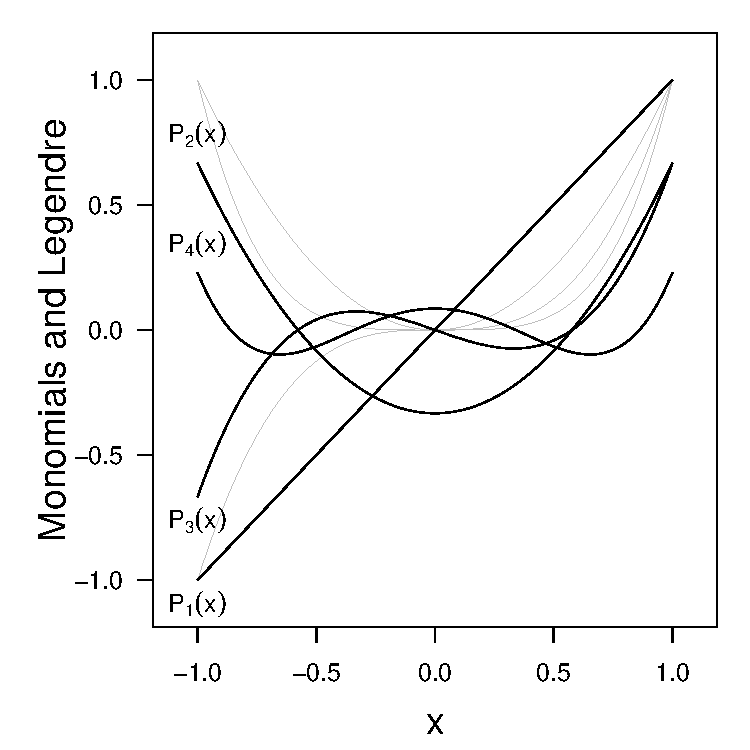
\includegraphics[width=\textwidth]{3_approximation/legendre_funs.pdf}

\end{minipage}
\begin{minipage}[c]{0.48\textwidth}
\begin{align*}
P_0(x) & = 1\\
P_1(x) & = x\\
P_2(x) & = x^2-\dfrac{1}{3}\\
P_3(x) & = x^3-\dfrac{3}{5}x\\
 & \dots\\
P_n(x) & = (x-B_k)P_{n-1}(x)-C_kP_{x-2}(x)
\end{align*}

where
\begin{align*}
B_k & = \dfrac{\int_{-1}^1 x \cdot 1 \cdot [P_{k-1}(x)]^2\,dx}{\int_{-1}^1 1 \cdot [P_{k-1}(x)]^2\,dx}\\
C_k & = \dfrac{\int_{-1}^1 x \cdot 1 \cdot [P_{k-1}(x) P_{k-2}(x)]\,dx}{\int_{-1}^1 1 \cdot [P_{k-2}(x)]^2\,dx}
\end{align*}

\caption{In gray the intuitive monomials \(\phi_i(x) = x^i\) with the Legendre polynomials \(P_i(x)\) in black.}\label{fig::leg}

\end{minipage}
\end{figure}

%%%%%%%%%%%%%%%%%%%%%%%%%%
%%%%%%%%%%%%%%%%%%%%%%%%%%
\subsubsection{Chebyshev polynomials}
The standard monomials for function approximation, shown as the familiar unlabeled gray curves in Figure~\ref{fig::cheb}, are \(\phi_i(x) = x^i\) for \(i=0, 1, \dots, n\). These lack the property of orthogonality that is achieved by the Chebyshev polynomials, also shown Figure~\ref{fig::cheb}, but in black and labeled. The first few Chebyshev polynomials are
%
\begin{figure}[ht!]\centering

\begin{minipage}[c]{0.48\textwidth}
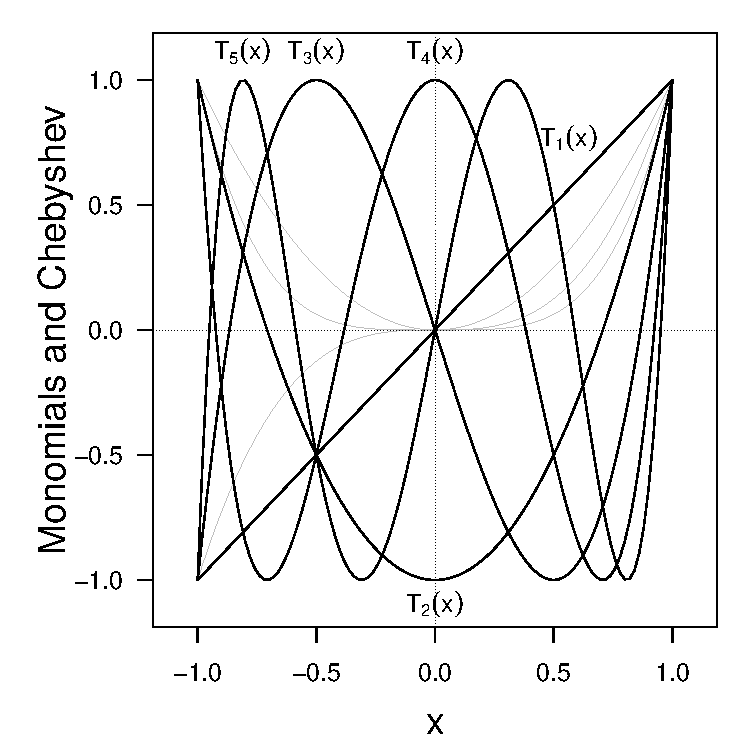
\includegraphics[width=\textwidth]{3_approximation/cheb_funs.pdf}

\end{minipage}
\begin{minipage}[c]{0.48\textwidth}
\begin{align*}
T_0(x) & = 1\\
T_1(x) & = x\\
T_2(x) & = 2x^2-1\\
T_3(x) & = 4x^3-3x\\
 & \dots\\
T_n(x) & = 2xT_{n-1}(x) - T_{n-2}(x)
\end{align*}

\caption{In gray the intuitive monomials \(\phi_i(x) = x^i\) with the Chebyshev polynomials \(T_i(x)\) in black.}\label{fig::cheb}

\end{minipage}
\end{figure}

Since the alternate definition of the Chebyshev polynomials is \(T_n(x) = \cos(n\arccos(x))\) for \(n\geq0\), it should seem reasonable that these functions are bounded in magnitude by one, as illustrated in Figure~\ref{fig::cheb}. The monic Chebyshev polynomials (not illustrated, but handy for Chebyshev economization of power series), with leading coefficient \(1\), are defined by \[\tilde T_n(x) = \dfrac{1}{2^{n-1}}T_n(x)\] For these polynomials the extrema, which occur \textit{at} the same points, are those of \(T_n(x)\) but reduced in value by a factor of \(\dfrac{1}{2^{n-1}}\), that is, the extrema are, for \(k=0, 1, \dots, n\) \[\tilde T'_n(\bar x_k) = \dfrac{(-1)^k}{2^{n-1}}\]


%%%%%%%%%%%%%%%%%%%%%%%%%%
%%%%%%%%%%%%%%%%%%%%%%%%%%
\subsubsection{Chebyshev points and Lagrange nodes}
By a theorem, we have that the optimal choice of nodes for polynomial approximation by a degree \(n\) polynomial is given by the zeros of of the \((n+1)^\text{st}\) Chebyshev polynomial \(T_{n+1}(x)\). For example, as given in Figure~\ref{fig::cheb_pts}, we take the approximation of \(f(x) = e^x\) on \([0, 1]\) with three points. We expect to to take, \(\tilde x_0 = 0\), \(\tilde x_1 = 0.5\), and \(\tilde x_2 = 1.0\), but achieve better performance with Chebyshev nodes \(\bar x_i\). The nodes for interpolation are given by the zeros of the Chebyshev polynomial \(T_3(x)\), which in turn are given by \(\bar x_k = \cos\left(\dfrac{2k-1}{2n}\pi\right)\) for \(k=1, 2, 3\).
\begin{align*}
\bar x_1 &= \cos\left(\dfrac{2(1)-1}{2(3)}\cdot\pi\right) = \cos\left(\dfrac{1\cdot\pi}{6}\right)= \dfrac{\sqrt{3}}{2} ~\approx~ 0.866\\
\bar x_2 &= \cos\left(\dfrac{2(2)-1}{2(3)}\cdot\pi\right) = \cos\left(\dfrac{3\cdot\pi}{6}\right)= 0\\
\bar x_3 &= \cos\left(\dfrac{2(3)-1}{2(3)}\cdot\pi\right) = \cos\left(\dfrac{5\cdot\pi}{6}\right)= -\dfrac{\sqrt{3}}{2} ~\approx~ -0.866 
\end{align*}

From \(\tilde x_i \in [a,b]\) we can compute \(\bar x_i \in [-1, 1]\) by \[x_i = \dfrac{2\tilde x_i - a - b}{b-a}\] and in the reverse we can use \[\tilde x_i = \dfrac{1}{2}\left((b-a)\bar x_i + a + b\right)\] As an example,
\begin{center}
\begin{tabular}{cll}
\(i\) & \(\phantom{-}\bar x_i\) & \(\tilde x_i\)\\
\hline \hline
& & \\[-10pt]
1 & \(\phantom{-}0.866\) & 0.933\\ 
2 & \(\phantom{-}0.0\) & 0.500 \\
3 & \(-0.866\) & 0.067
\end{tabular}
\end{center}

The n\"aively chosen nodes that include the endpoints (red) are illustrated in the left-hand panel of Figure~\ref{fig::cheb_pts}, and as shown give a reasonable approximate. Yet, the approximation is improved by use of the Chebyshev points (blue). 
%
\begin{figure}[ht!]\centering
\begin{minipage}{0.48\textwidth}
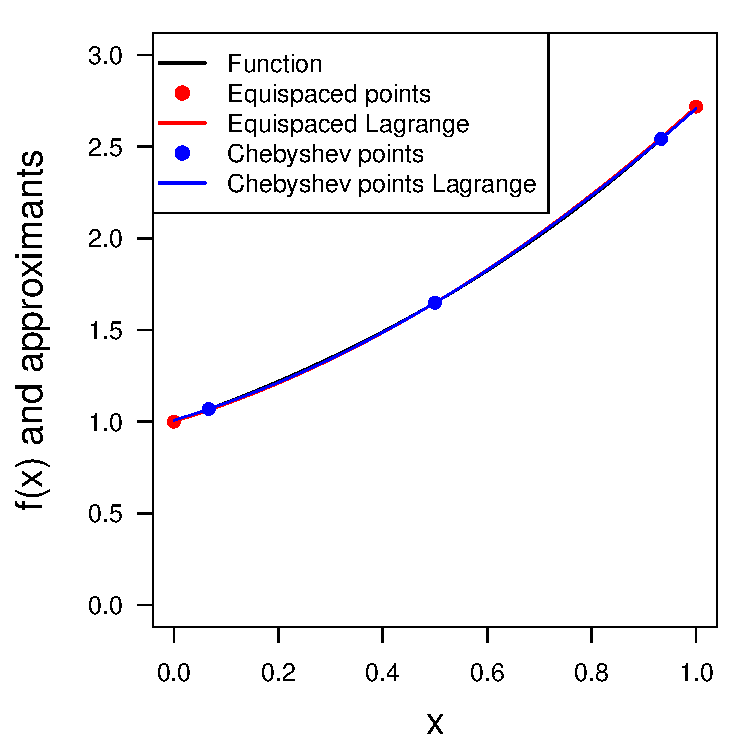
\includegraphics[width=\textwidth]{3_approximation/cheb_pts_lagr.pdf}

\end{minipage}
\begin{minipage}{0.48\textwidth}

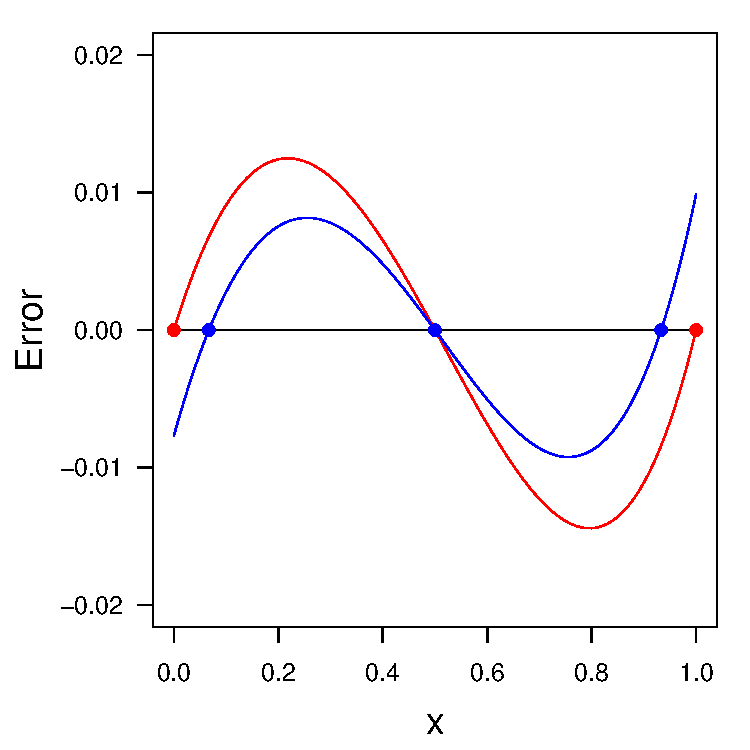
\includegraphics[width=\textwidth]{3_approximation/cheb_pts_lagr_err.pdf}

\end{minipage}
\caption{Lagrange interpolation of \(f(x) = e^x\) on \([0,1]\), but with Chebyshev points instead of equispaced points.}\label{fig::cheb_pts}
\end{figure}
%
Notice, from Figure~\ref{fig::cheb_zeros}, that the zeros accumulate or cluster near the boundary of the interval. This helps to `clamp down' the polynomial interpolation near the boundary.
%
\begin{figure}[ht!]\centering

\begin{minipage}[c]{0.48\textwidth}
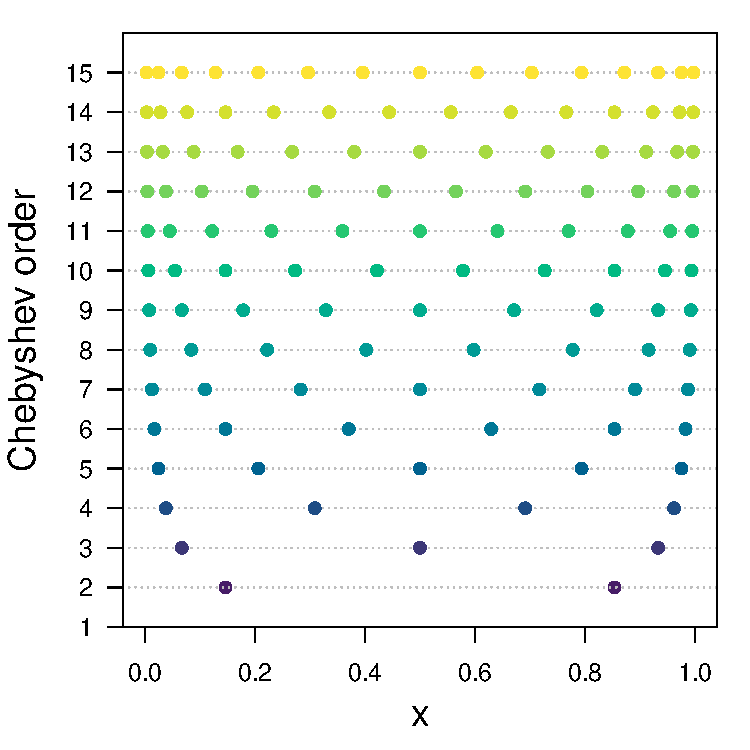
\includegraphics[width=\textwidth]{3_approximation/cheb_zeros.pdf}

\end{minipage}
\begin{minipage}[c]{0.48\textwidth}

\caption{Location of zeros to \(T_n(x)\) in the interval \([0, 1]\) for Chebyshev functions of orders from \(n=2, 3, \dots, 15\).}\label{fig::cheb_zeros}

\end{minipage}
\end{figure}


%%%%%%%%%%%%%%%%%%%%%%%%%%
%%%%%%%%%%%%%%%%%%%%%%%%%%
\subsubsection{Chebyshev economization}
As we will soon see, the `best' reduced order polynomial approximation \(P_{n-1}\) to a polynomial \(P_n(x)\) is given by \[P_{n-1}(x) = P_{n}(x) - a_n\tilde T_n(x)\] where \(\tilde T_n(x)\) is the \(n^\text{th}\) order monic Chebyshev polynomial and \(a_n\) is the coefficient of the highest order term in \(P_n(x)\). To economize the polynomial approximation to \(f(x) = e^x\) given by a \(4^\text{th}\) order Maclaurin polynomial, we can subtract \(\dfrac{1}{24}\tilde T_4(x)\) from the original \(P_4(x)\) (note that \(a_4=\dfrac{1}{24}\) in the original polynomial representation). This alters coefficients of all powers of \(x\) of lower orders that are present in \(T_4(x)\) and eliminates the \(4^\text{th}\) order term entirely. Notice in Figure~\ref{fig::cheb_ord} that the maximum error for the third order function is only slightly worse for \(x=1.0\) than for the fourth order function.

\begin{figure}[ht!]\centering
\begin{minipage}{0.48\textwidth}
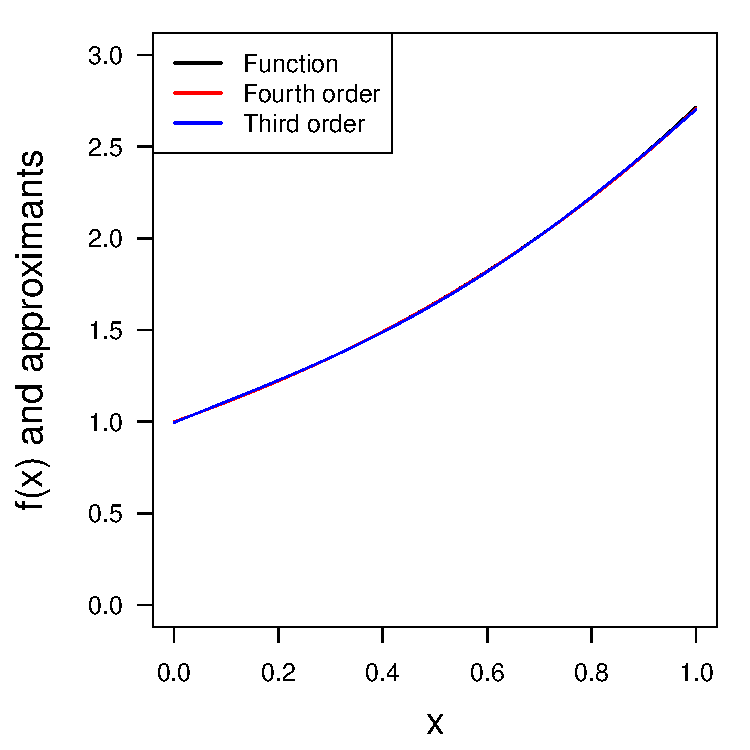
\includegraphics[width=\textwidth]{3_approximation/cheb_order_lagr.pdf}

\end{minipage}
\begin{minipage}{0.48\textwidth}

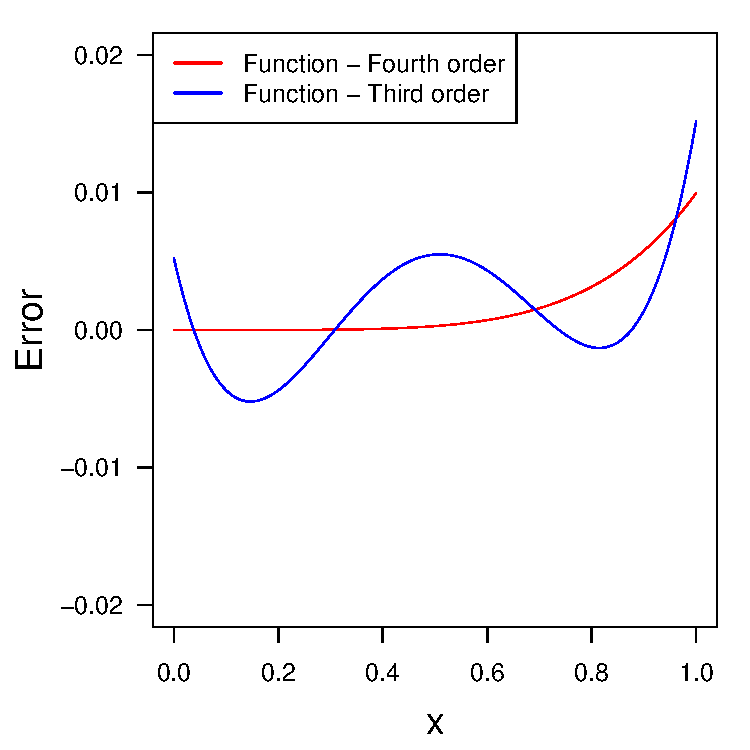
\includegraphics[width=\textwidth]{3_approximation/cheb_order_lagr_err.pdf}
\end{minipage}
\caption{Left: Full- and reduced-order approximations of \(f(x) = e^x\) on \([0, 1]\) by \(P_3(x)~=~P_4(x)~-~a_4 \tilde T_4(x)\). Right: Error in approximations of \(f(x) = e^x\) by full- and reduced-order polynomials.}\label{fig::cheb_ord}
\end{figure}

%%%%%%%%%%%%%%%%%%%%%%%%%
\clearpage
\section{Numerical calculus}
\subsection{Numerical differentiation}
Consider the function \(f(x) = e^x\) at a point \(x_0=1\) and approximations to its derivative \(f'(x_0)~\approx~ 2.71281\). Approximations can be made by to somewhat straightforward approximations: the first-order forward difference and the second-order forward and centered differences. The error in these approximations is illustrated below, with rounding to simulate calculations by single-precision and double-precision numbers.

\begin{figure}[ht!]\centering
\begin{minipage}{0.48\textwidth}
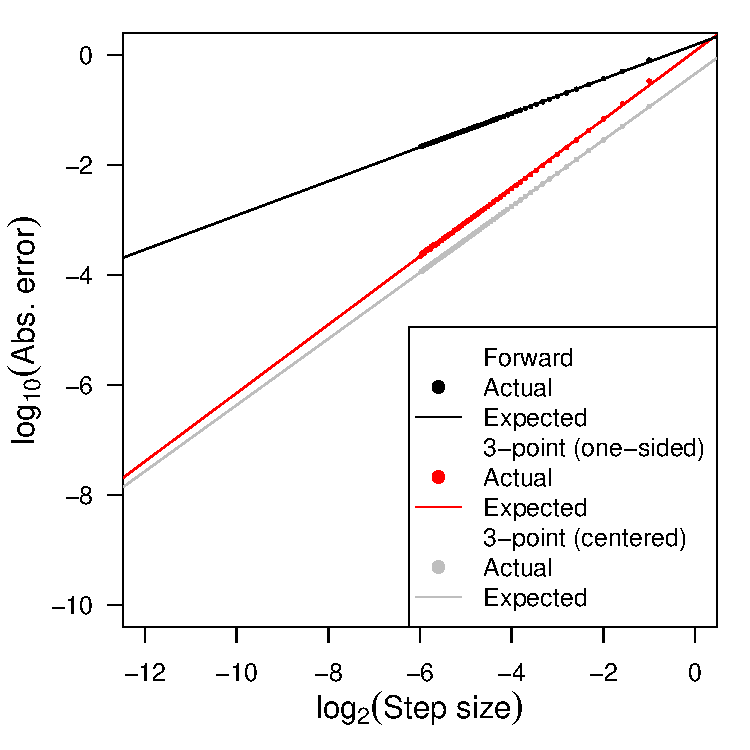
\includegraphics[width=0.9\textwidth]{4_differentiation/step_size_8.pdf}

\end{minipage}
\begin{minipage}{0.48\textwidth}
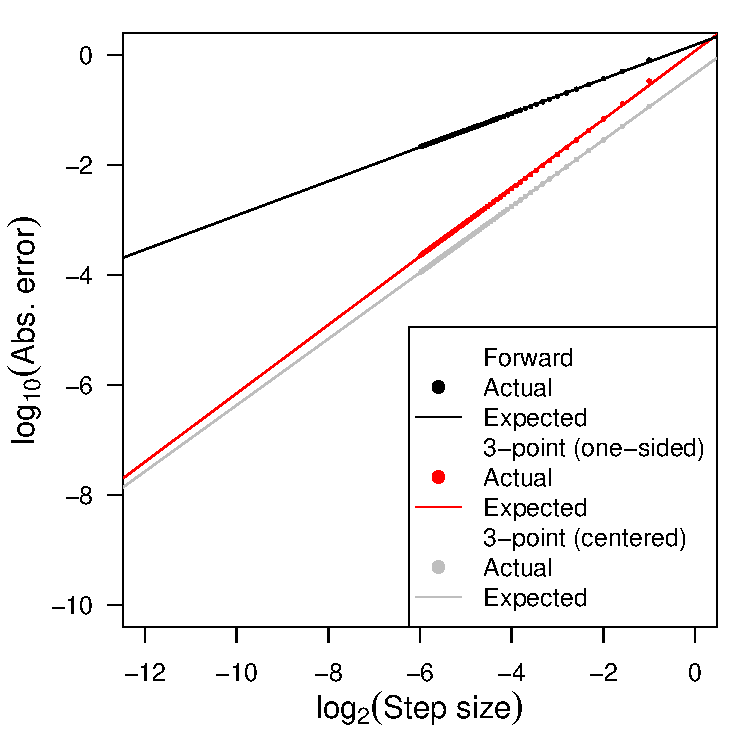
\includegraphics[width=0.9\textwidth]{4_differentiation/step_size_16.pdf}

\end{minipage}

\caption{Points indicate calculated \(\log_{10}\left(\text{abs. error}\right)\) for first-order forward (black), second-order forward (red), and centered (gray) difference approximations. Line illustrates predicted reduction in error as step size shrinks. \textbf{Left:} 8 digit calculation (simulated single-precision), \textbf{Right:} 16 digit calculation (simulated double-precision)}\label{fig::plots}
\end{figure}
%

\begin{figure}[ht!]\centering
\begin{minipage}{0.48\textwidth}
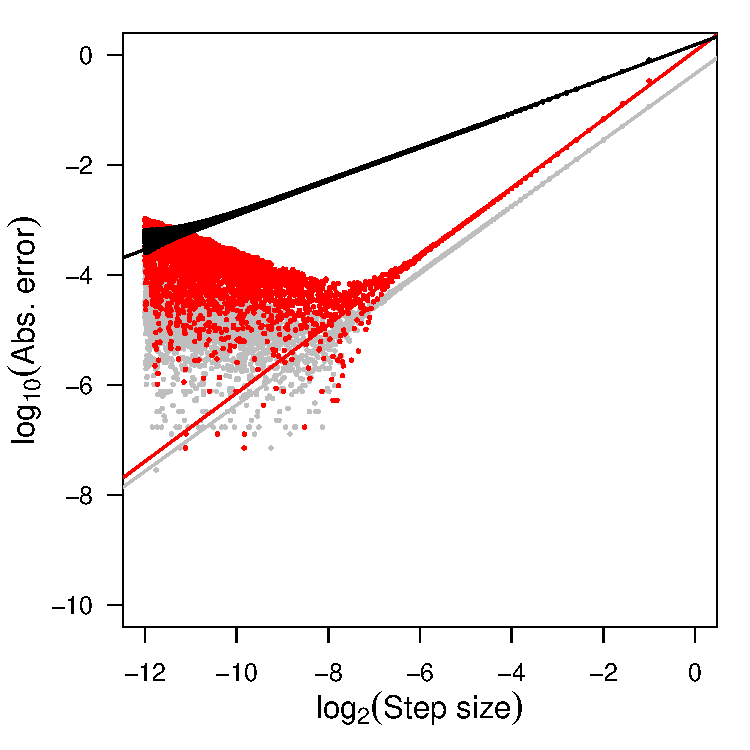
\includegraphics[width=0.9\textwidth]{4_differentiation/step_size_roundoff_8.pdf}

\end{minipage}
\begin{minipage}{0.48\textwidth}
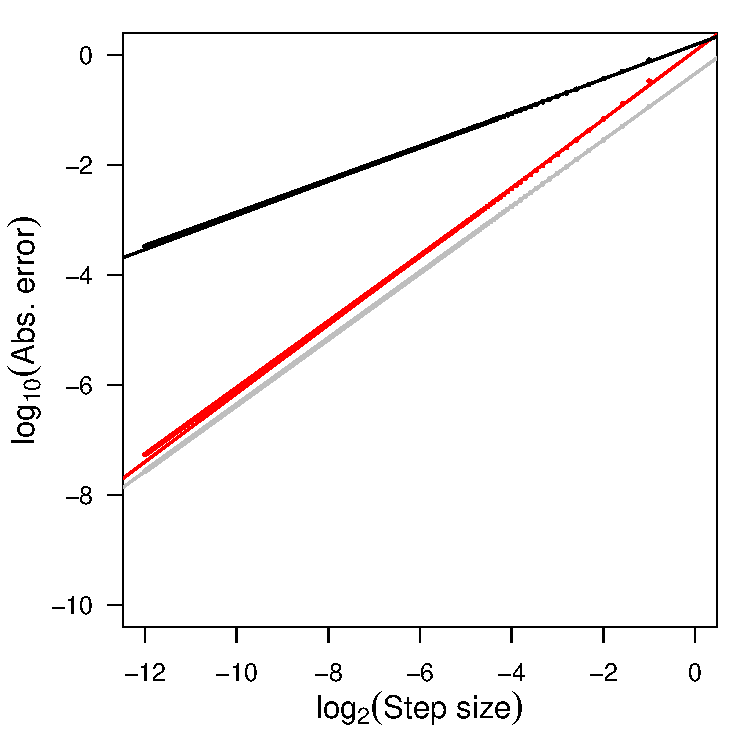
\includegraphics[width=0.9\textwidth]{4_differentiation/step_size_roundoff_16.pdf}
\end{minipage}

\caption{As in Figure~\ref{fig::plots}, but with smaller step sizes included. Note that error \textit{increases} due to roundoff for both methods, but especially for the centered method as the step size is reduced below \(h = 0.01\).}\label{fig::roundoff}
\end{figure}


\clearpage
\subsection{Numerical integration (Monte Carlo)}
\textit{This section may be imperfect, but reflects the main idea.}

Though not emphasized here, the techniques that follow are most useful in higher dimensional integrals. We can integrate \(f(x) = x^2\) using the Fundamental Theorem of Calculus,
\[\int_0^2 x^2\,dx = \left.\left(\dfrac{x^3}{3}\right)\right|_0^2 = \dfrac{2^3}{3} - \dfrac{0^3}{3} = \dfrac{8}{3}\]
From the Mean Value Theorem for Integrals we have that \[\hat{f} = \dfrac{1}{2-0}\int_0^2 x^2\,dx = \dfrac{1}{2}\cdot \dfrac{8}{3} = \dfrac{4}{3}\]
The shaded region on the left panel (Fig~\ref{fig::calc}) shows the area under the curve. The area on the right is the same size, but bounded by a constant function whose value is \(\hat{f}\).

\begin{figure}[h!]\centering
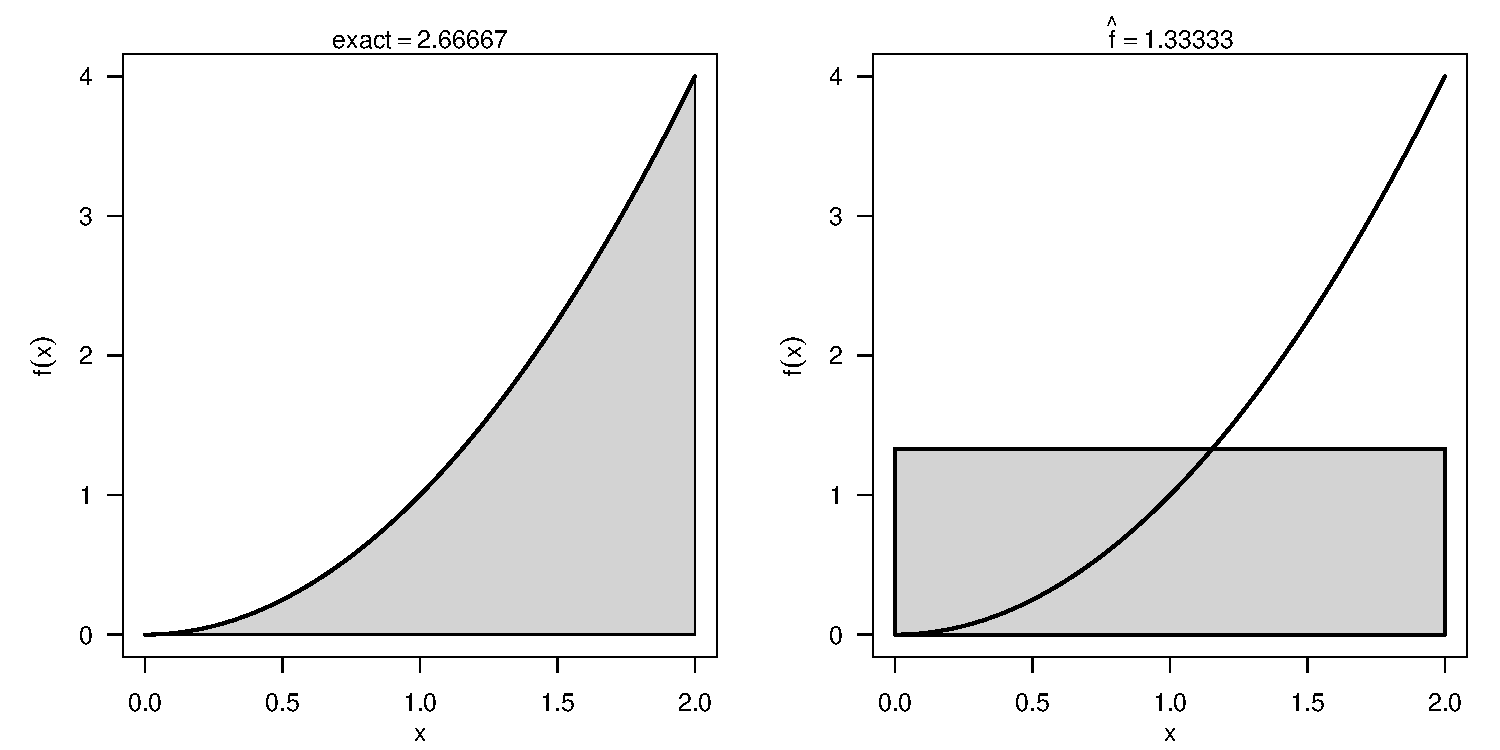
\includegraphics[width=0.9\textwidth]{5_integration/intro.pdf}
\caption{Left: Traditional calculus interpretation of the area under the curve. Right: Average value of a function defined by equal area.}\label{fig::calc}
\end{figure}

One scheme of Monte Carlo integration uses function values at randomly chosen points to calculate areas which are then averaged. Here \[\int_a^b f(x)\,dx \approx \dfrac{1}{N}\sum_{i=1}^{N} \underbrace{(b-a)f(x_i)}_\text{\(i\)th area} = (b-a)\underbrace{\dfrac{1}{N}\sum_{i=1}^{N} f(x_i)}_\text{average height}\] Fig~\ref{fig::average} (left panel) shows 5 of the 100 random rectangle regions. The shaded area on the right panel corresponds to the region whose height is the average of the random function values. Notice that this height very closely compares with the average value of the function, thus the areas of the regions are similar.
%
\begin{figure}[h!]\centering
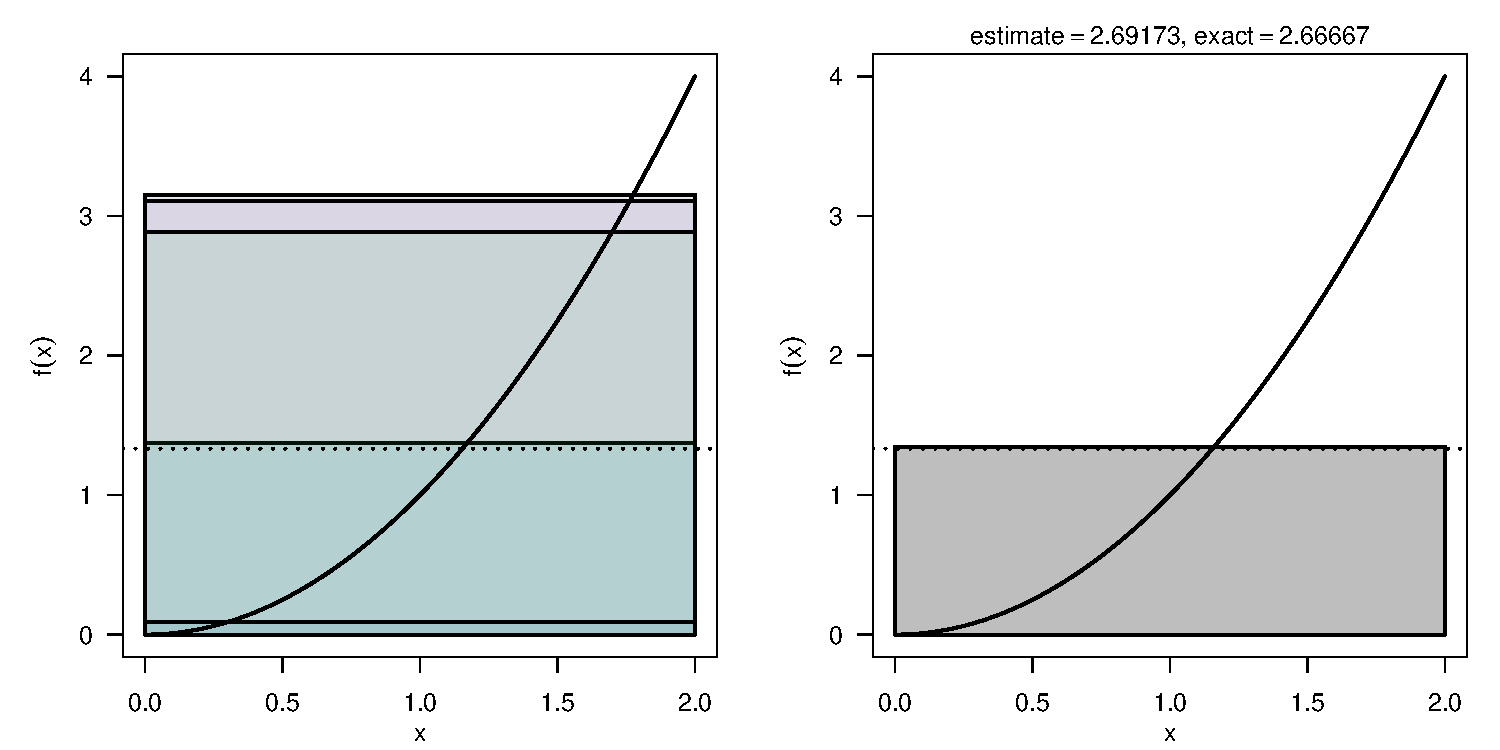
\includegraphics[width=0.9\textwidth]{5_integration/rectangles.pdf}
\caption{Dashed line indicates \(\hat{f}\) from traditional calculus. Left: 5 sample rectangles (shaded). Right: Average area and function height by random sampling.}\label{fig::average}
\end{figure}

An alternate scheme (Fig~\ref{fig::compare}, left) plots points in the plane and considers the fraction of points that fall below the curve (i.e., `the acceptance region`). This fraction is multiplied by the total area of the region (easier to calculate since the shape is likely square). Though this is easier to program than the notation might suggest, consider the indicator function \[I(i) = \begin{cases}1, \quad y_i < f(x_i)\\0, \quad\text{otherwise}\end{cases}\]~and take~\[\int_a^b f(x)\,dx \approx(f_{max}-f_{min})(b-a)\dfrac{1}{N} \sum_{i=1}^N I(i)\]
%
\begin{figure}[h!]\centering
\begin{minipage}{0.48\textwidth}\centering
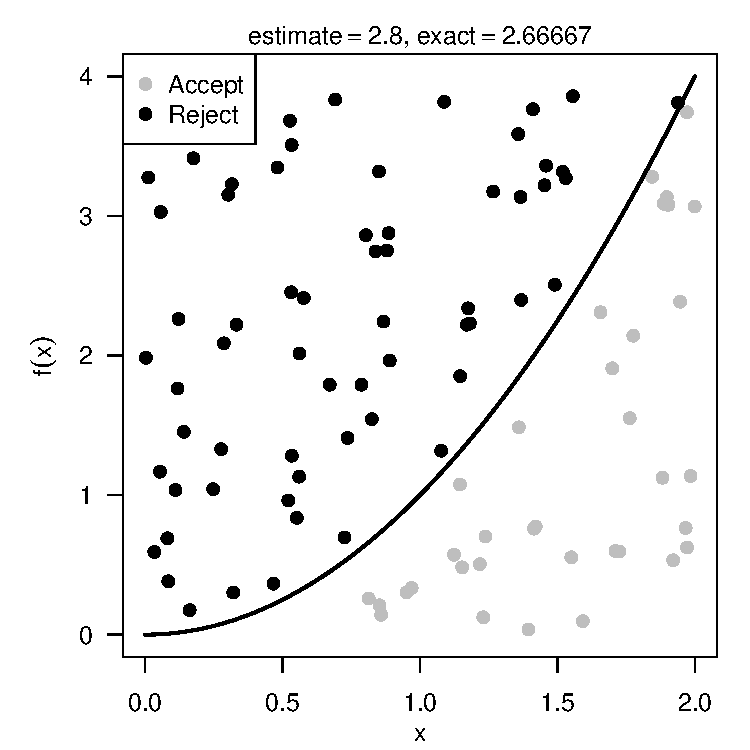
\includegraphics[width=0.9\textwidth]{5_integration/rejection.pdf}

\end{minipage}
\begin{minipage}{0.48\textwidth}

\centering
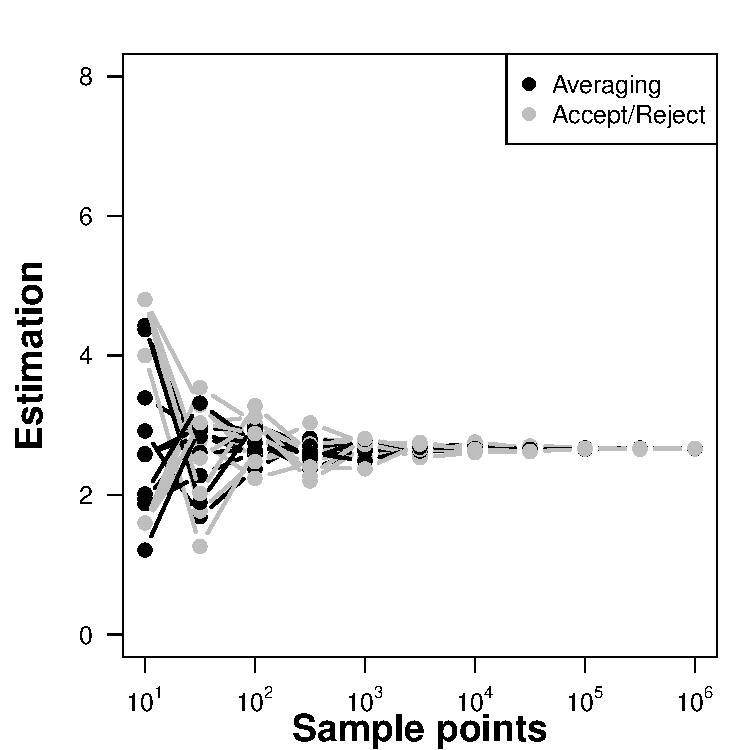
\includegraphics[width=0.9\textwidth]{5_integration/Ns.pdf}
\end{minipage}
\caption{Left: Accepted points fall below the graph of the function. Right: Comparison of rectangle method and rejection method for ten different trials of each.}\label{fig::compare}
\end{figure}


\end{document}